%% paper.tex — Testing for Simplicial Geometry
%% arXiv preprint targeting Random Structures and Algorithms (Wiley)
%% Compile: cd simplicial-latent-geometry/my_theorems && pdflatex paper && bibtex paper && pdflatex paper && pdflatex paper

\documentclass[reqno,12pt]{amsart}

%% ── Encoding & fonts ─────────────────────────────────────────────────────────
\usepackage[utf8]{inputenc}
\usepackage[T1]{fontenc}
\usepackage{microtype}

%% ── Mathematics ──────────────────────────────────────────────────────────────
\usepackage{amsmath,amssymb,amsthm}
\usepackage{mathtools}          % \coloneqq, dcases

%% ── Bibliography ─────────────────────────────────────────────────────────────
\usepackage[numbers,sort&compress]{natbib}

%% ── Hyperlinks ───────────────────────────────────────────────────────────────
\usepackage[dvipsnames,svgnames,x11names]{xcolor}
\usepackage[colorlinks=true,
            linkcolor=RoyalBlue4,
            citecolor=RoyalBlue4,
            urlcolor=NavyBlue]{hyperref}
\usepackage{url}

%% ── Page geometry ────────────────────────────────────────────────────────────
\usepackage[top=1in,bottom=1in,left=1in,right=1in]{geometry}

%% ── Enumitem for tighter lists ───────────────────────────────────────────────
\usepackage{enumitem}

%% ── Figures ──────────────────────────────────────────────────────────────────
\usepackage{tikz}

%% ─────────────────────────────────────────────────────────────────────────────
%%  MACROS
%% ─────────────────────────────────────────────────────────────────────────────

%% Models and statistics
\newcommand{\tauf}{\tau_{\mathrm{f}}}
\newcommand{\tauff}{\tau_{\mathrm{ff}}}
\newcommand{\PC}{\mathrm{2PC}}
\newcommand{\Cech}{\ifmmode\text{\v{C}ech}\else\v{C}ech\fi}  % Čech (text+math)
\newcommand{\RGG}{\mathrm{RGG}}
\newcommand{\TV}{\mathrm{TV}}

%% Named quantities
\newcommand{\geomCov}{\mathrm{geomCov}}
\newcommand{\fillingP}{\mathrm{fillingProb}}
\newcommand{\matchR}{\mathrm{matchRadius}}

%% Sets and spaces
\newcommand{\TT}{\mathbb{T}}         % flat torus
\newcommand{\AddCircle}{\mathbb{T}^1}% AddCircle(1) = ℝ/ℤ, the unit circle
\newcommand{\RR}{\mathbb{R}}
\newcommand{\NN}{\mathbb{N}}
\newcommand{\ZZ}{\mathbb{Z}}
\newcommand{\Sph}{\mathbb{S}}

%% Probability
\newcommand{\EE}{\mathbb{E}}
\newcommand{\PP}{\mathbb{P}}
\DeclareMathOperator{\Var}{Var}
\DeclareMathOperator{\Cov}{Cov}

%% Lean annotation (gray box for theorem names)
\newcommand{\lean}[1]{\textup{\texttt{\small #1}}}
\newcommand{\leanverified}[1]{\textup{(Lean: \texttt{#1}, 0 sorries)}}


%% ─────────────────────────────────────────────────────────────────────────────
%%  THEOREM ENVIRONMENTS
%% ─────────────────────────────────────────────────────────────────────────────

\theoremstyle{plain}
\newtheorem{theorem}{Theorem}[section]
\newtheorem{lemma}[theorem]{Lemma}
\newtheorem{proposition}[theorem]{Proposition}
\newtheorem{corollary}[theorem]{Corollary}

\theoremstyle{definition}
\newtheorem{definition}[theorem]{Definition}
\newtheorem{observation}[theorem]{Observation}
\newtheorem{example}[theorem]{Example}

\theoremstyle{remark}
\newtheorem{remark}[theorem]{Remark}
\newtheorem{conjecture}[theorem]{Conjecture}

%% ─────────────────────────────────────────────────────────────────────────────
%%  DOCUMENT
%% ─────────────────────────────────────────────────────────────────────────────

\begin{document}

\title[Testing for Simplicial Geometry]{Testing for Simplicial Geometry: A Signed Triangle
  Statistic for the \v{C}ech--2PC Phase Transition}

\author[Goh and Cook]{David Goh\textsuperscript{$\star$}}
\address{\textsuperscript{$\star$}Department of Computer Science, University of Toronto}
\email{daveed@cs.toronto.edu}

\author{Nicholas A.\ Cook\textsuperscript{$\ddagger$}}
\thanks{${}^{\ddagger}$ Supported in part by NSF grant DMS-2154029.}
\address{\textsuperscript{$\ddagger$}Department of Mathematics, Duke University, Durham, NC, USA}
\email{nicholas.cook@duke.edu}

\date{}

\subjclass[2020]{%
  Primary 05C80 (random graphs, generic models);
  Secondary 55U10 (simplicial sets and complexes),
  62H30 (classification and discrimination; cluster analysis).}

\keywords{random simplicial complex, geometry detection, Čech complex, signed triangle statistic,
  phase transition, Lean 4, formal verification}

\begin{abstract}
We study the geometry detection problem for random 2-dimensional simplicial complexes:
distinguish the \emph{2-parameter null} $\PC(n,p,q)$---in which edges and triangle fills
are independent---from a geometric alternative built on $n$ iid points in a latent ambient
space, with edges and fills determined by proximity. We introduce the
\emph{doubly-signed filled triangle statistic} $\tauf$, the natural simplicial analogue of
the BDER signed triangle, centered with respect to both edge and fill indicators. Under
$\PC$, $\tauf$ has mean zero and variance $\Theta(n^3)$; under any matched geometric model,
$\EE[\tauf] = \binom{n}{3}\cdot\geomCov(p,d)$.

The paper bundles two complementary instances of this framework, organized by the
\emph{Helly number} of the ambient space.

\smallskip
\noindent\textbf{Paper~1 (Helly-2: $\ell^\infty$ torus, Rips clique fill).}
On $\TT^d$ with the sup-norm, the Helly-2 property of the circle collapses any \v{C}ech
existential nerve onto its Rips clique fill, so the natural downward-closed simplicial
model is the Rips clique complex with $F_{ijk} = A_{ij} A_{ik} A_{jk}$. In this regime
there is \emph{no $n$-independent dimensional barrier}: for fixed $p \in (0,1)$,
$\geomCov(p,d) \to p^3(1-p)^3 > 0$ as $d \to \infty$, and detection succeeds for every
fixed~$d$.

\smallskip
\noindent\textbf{Paper~2 (Helly-$d$: sphere $S^{d-1}$, proper \v{C}ech fill).}
On the sphere, Helly's theorem preserves the genuine \v{C}ech-vs.-Rips distinction.
A Wishart-derived joint Gram-entry density of order $(\det G)^{(d-4)/2}$ gives the
super-exponential tail
$1 - q_{\text{\v{C}ech}}(p,d) \sim (3 z_p^2 / d)^{(d-2)/2}$, where $z_p = \Phi^{-1}(1-p)$.
The detection threshold is sub-logarithmic:
$d^*(n,p) = 3 \log n / \log\log n$, with universal leading constant~$3$.

\smallskip
\noindent\textbf{Methodology.} The Helly number of the ambient space is the
discriminator: Helly-2 ambients exhibit no dimensional barrier (the existential nerve
collapses), while Helly-$d$ ambients (e.g.\ the sphere) preserve a genuine $d$-dependent
barrier. The moment chain, the Paley--Zygmund detection bound (Paper~1 headline
\lean{phase\_transition}), and the regime-free Rips closed form
$\geomCov(p,d) = q[(1-p)^3 + p^3] - q^2$ with limit $p^3(1-p)^3$ are formally verified in
Lean~4 with Mathlib~\cite{Mathlib2020}, with no sorries in the active proof chain;
the sphere headline reduces to six explicitly named structural axioms.
\end{abstract}

\maketitle

%% ─────────────────────────────────────────────────────────────────────────────
\section{Introduction}\label{sec:intro}
%% ─────────────────────────────────────────────────────────────────────────────

\subsection{Background and Motivation}

Topological data analysis (TDA) infers the shape of data by building simplicial complexes on
point clouds and measuring their homology. The foundational pipeline---sample $n$ points, form
the \v{C}ech or Vietoris-Rips complex at radius $r$, read off Betti numbers or persistent
homology---rests on the assumption that observed topological features reflect genuine geometry
in the underlying data. But any finite point cloud will produce some triangles and higher faces
by chance; the practical question is whether those topological features are signal or noise.

\medskip
\noindent\textbf{The Helly-discriminator framing.}
The detection landscape for geometric simplicial complexes depends sharply on the
\emph{Helly number} of the latent ambient space. The \v{C}ech complex is defined by the
existential nerve criterion (a triple fills when its three balls share a common point);
the Rips complex is defined by the clique criterion (a triple fills when all three pairwise
edges are present). On ambients with Helly number~$2$---such as the circle, hence the
$\ell^\infty$ torus by coordinatewise factorisation---these two definitions
\emph{coincide as set complexes}: a triple of pairwise-intersecting balls necessarily has a
common point. The natural downward-closed simplicial model in this regime is the Rips
clique complex, and there is no $n$-independent dimensional barrier on $\TT^d$.
On ambients with Helly number~$d$---such as the sphere $S^{d-1}$---the existential nerve
genuinely strengthens the clique condition, and the gap between the two complexes survives
concentration of measure, supporting a genuine sub-logarithmic dimensional barrier.

This paper bundles the two regimes within a single framework. Paper~1
(\S\S\ref{sec:linfty-statistic}--\ref{sec:linfty-detection}) handles
the Helly-2 case: $\ell^\infty$ torus with Rips clique fill, no dimensional barrier,
$\geomCov \to p^3(1-p)^3 > 0$. Paper~2 (\S\ref{sec:sphere-instance}, with full Wishart
derivation in Appendix~\ref{app:wishart}) handles the Helly-$d$ case: sphere with proper
\v{C}ech fill, sub-logarithmic threshold $d^*(n,p) = 3 \log n / \log\log n$.
Section~\ref{sec:helly-discriminator} states the unifying observation: the existence (or
absence) of an $n$-independent dimensional barrier is determined by whether the ambient
admits a \emph{global candidate witness} for the \v{C}ech existential.

\paragraph{Acknowledgment of reframe.}
An earlier draft of the $\ell^\infty$-torus instance was formulated around a same-radius
``\v{C}ech'' fill (triple-ball intersection at radius $r$) which is not downward-closed
when edges are defined by $d_\infty \le r$. N.~Cook (May~2026) diagnosed this as a
Helly-2 algebraic collapse rather than a structural barrier; the present bundle follows
his diagnosis by replacing the existential nerve with the Rips clique on the torus while
preserving the existential nerve on the sphere, where Helly-$d$ keeps it honest.

Kahle~\cite{Kahle2011} systematically studied the expected topology of \v{C}ech and
Vietoris-Rips complexes built on i.i.d.\ random points in $\RR^d$, establishing connectivity
and component-count thresholds as higher-dimensional analogues of results for random geometric
graphs. A central motivation, surveyed in Bobrowski and Kahle~\cite{Bobrowski2018}, is the
need for probabilistic null hypotheses against which TDA test statistics can be calibrated;
the random geometric complex on i.i.d.\ uniform points is the natural geometric alternative
to such a null.

The simplest null model for 2-dimensional complexes is the \emph{2-parameter complex}
$\PC(n,p,q)$: place $n$ vertices, insert each edge independently with probability $p$, and
fill each completed triangle independently with probability $q$ (see also the multi-parameter
model of Kahle~\cite{Kahle2016}). This encodes no geometry---all events are mutually
independent. The geometric alternative is the \emph{\v{C}ech complex} $\Cech(n,r,d)$: sample
$n$ points uniformly on the flat torus $\TT^d$, connect two points whenever they lie within
distance $r$, and fill a triangle whenever the three associated sup-norm balls of radius $r$
share a common point (the nerve criterion~\cite{Bjorner1995}; see also
Figure~\ref{fig:models}). The fundamental detection question is: given only
the observed simplicial complex, can one tell which model generated it?

\subsection{Related Work}\label{sec:related}

\subsubsection*{Geometry testing for random graphs}
Bubeck, Ding, Eldan, and R\'acz~\cite{Bubeck2016} introduced the signed triangle statistic
for testing $G(n,p)$ vs.\ $\RGG(n,p,d)$ on $\Sph^{d-1}$, establishing the $d\asymp n^3$
phase transition: random geometric graphs are detectable when $d\ll n^3$ and
indistinguishable from Erd\H{o}s--R\'enyi when $d\gg n^3$. Bangachev and
Bresler~\cite{BangachevBresler2024} studied the low-degree Fourier coefficients of random
geometric graphs on $\Sph^{d-1}$, showing that the signed triangle statistic is
computationally optimal for this testing problem and characterizing the Fourier coefficient
behavior across the full range of densities. Liu, Mohanty, Schramm, and Yang~\cite{Liu2022}
obtained sharp detection thresholds for sparse random geometric graphs via the low-degree
polynomial framework; their methods provide a model for sharpening the SNR condition below the
detection threshold. Brennan, Bresler, and Huang~\cite{Brennan2022} extended BDER to
anisotropic latent geometries; a complementary line due to Litvak, Michielan, and
Stegehuis~\cite{Litvak2022} shows that triangle-count statistics are insufficient to detect
\emph{hyperbolic} geometry in networks, underscoring that the power of triangle-based tests
is geometry-dependent. Perkins~\cite{Perkins2024} surveys recent progress on sharp
thresholds in random structures.
Our work carries this framework into the simplicial setting, where the presence of fill
indicators introduces an additional layer of geometric dependence beyond edge structure alone.
The detection landscape splits along the Helly number of the latent ambient. On Helly-2
ambients (the $\ell^\infty$ torus, Paper~1), the Rips clique fill is structurally aligned
with the edge layer and the per-triangle signal $\geomCov(p,d)$ stabilises at
$p^3(1-p)^3 > 0$ as $d \to \infty$, giving no $n$-independent barrier and recovering a
BDER-style SNR threshold. On Helly-$d$ ambients (the sphere, Paper~2), the existential
\v{C}ech fill genuinely strengthens the clique condition and the signal vanishes
super-exponentially in~$d$, giving the sub-logarithmic $d^*(n,p) = 3\log n / \log\log n$.

\subsubsection*{Hypergraph detection}
Dhawan, Mao, and Wein~\cite{DhawanMaoWein2023} study detection of planted dense
subhypergraphs via low-degree polynomials in $r$-uniform hypergraphs, establishing sharp
thresholds in the log-density regime. Their setting is combinatorial (planted structure in an
Erd\H{o}s--R\'enyi null) rather than geometric, but the low-degree framework and the
connection between hyperedge counting statistics and the structure of test polynomials is
closely related to our context. We view their analysis as the combinatorial cousin of our
geometric detection problem: the 2PC null here plays the role of their Erd\H{o}s--R\'enyi
hypergraph, and the \v{C}ech complex plays the role of their planted dense substructure,
but the source of dependence (latent torus positions rather than a planted clique) is
qualitatively different and yields a different class of tests.

\subsubsection*{Random geometric complexes and TDA}
Kahle~\cite{Kahle2011} established homology thresholds for \v{C}ech and Vietoris-Rips
complexes on random points in $\RR^d$, motivated by the need for null models in TDA.
Kahle~\cite{Kahle2016} surveys the multi-parameter model $X(n;p_1,p_2,\ldots)$ (of which
our $\PC(n,p,q)$ is a special case) and the connection to persistent homology.
Bobrowski and Kahle~\cite{Bobrowski2018} survey random geometric complexes, explicitly
connecting the topology of such complexes to null hypotheses for topological statistics.
Tem\v{c}inas, Nanda, and Reinert~\cite{Temcinas2025} develop goodness-of-fit tests for
the multi-parameter random simplicial complex $\mathbf{X}(n,\mathbf{p})$ in the dense
regime, using multivariate CLTs for subcomplex counts proved via Stein's method.
Their setting and ours are complementary: they test a single null
$\mathbf{X}(n,\mathbf{p})$ against unspecified alternatives (one-sample goodness-of-fit),
while we formulate a two-sample detection problem between a combinatorial null
($\PC$) and a geometric alternative ($\Cech$). A technical point of contact is their
observation that raw subcomplex counts in $\mathbf{X}(n,\mathbf{p})$ have rank-one
limiting covariance, which motivates their switch to critical simplex counts from
discrete Morse theory; our doubly-signed $\tauf$ sidesteps this degeneracy directly
by centering both edge and fill indicators, yielding non-degenerate
$\Theta(n^3)$ variance under $\PC$ (Proposition~\ref{prop:moments-twopc}).
Tem\v{c}inas et al.\ also empirically demonstrate that their test can distinguish
$\mathbf{X}(n,\mathbf{p})$ from selected geometric simplicial complex models;
the present work gives a theoretical analogue with detection bounds on $\TT^d$
(Helly-2, no $n$-independent barrier) and a sub-logarithmic dimensional threshold
on $S^{d-1}$ (Helly-$d$).

\subsection{Main Results and Contributions}\label{sec:mainresults}

The key tool is the \emph{doubly-signed filled triangle statistic}
\begin{equation}\label{eq:tauf}
  \tauf = \sum_{\{i,j,k\}\in\binom{[n]}{3}}
    \Bigl[\prod_{e\in\partial\{i,j,k\}}(A_e - p)\Bigr](F_{ijk} - q),
\end{equation}
centered with respect to both edge and fill variability (Definition~\ref{def:tauf}).
The quantity $\geomCov(p,d)$ (Definition~\ref{def:geomcov}) is the per-triangle geometric-model
expectation of this doubly-centered product.

\medskip
\noindent\textbf{Paper~1: $\ell^\infty$ torus, Rips clique fill (Helly-2).}
On $\TT^d$ with sup-norm and Rips clique fill $F_{ijk} = A_{ij} A_{ik} A_{jk}$, the
regime-free closed form
\[
  \geomCov(p,d) = q\bigl[(1-p)^3 + p^3\bigr] - q^2, \qquad q = \fillingP(p,d),
\]
holds for all $p \in (0,1)$ and $d \ge 1$ (\lean{geometricCov\_eq}), giving the limit
$\geomCov(p,d) \to p^3 (1-p)^3 > 0$ as $d \to \infty$ at fixed $p$
(\lean{geometricCov\_tendsto\_pcubed\_compcubed}). Combined with the SNR calculation
(Lemma~\ref{lem:snr}) and the Paley--Zygmund Chebyshev pair, this yields the
detection theorem (Theorem~\ref{thm:detection}, \lean{detection\_lower\_bound\_fixed\_d}):
for every fixed $d \ge 1$, $\TV(\PC, \Cech_{\mathrm{Rips}}) \to 1$ as $n \to \infty$.
The joint-$(n,d)$ strengthening \lean{phase\_transition} extends this under an
asymptotic-equivalence hypothesis on $\geomCov$.

\medskip
\noindent\textbf{Paper~2: sphere $S^{d-1}$, proper \v{C}ech fill (Helly-$d$).}
Under the existential common-cap fill on $S^{d-1}$, the joint Gram-entry density
$\propto (\det G)^{(d-4)/2}$ (Wishart, Appendix~\ref{app:wishart}) yields the
super-exponential tail
\[
  1 - q_{\text{\v{C}ech}}(p,d)
  \sim \Bigl(\frac{3 z_p^2}{d}\Bigr)^{(d-2)/2},
  \qquad z_p = \Phi^{-1}(1-p),
\]
together with $\geomCov_{\text{\v{C}ech}}(p,d) = p^3 (1 - q_{\text{\v{C}ech}}(p,d))(1+o(1))$.
The detection threshold is sub-logarithmic:
$d^*(n,p) = 3 \log n / \log\log n$, with universal leading constant $3$.

\medskip
\noindent\textbf{Contributions.}
\begin{enumerate}[label=(\arabic*)]
\item \textbf{The doubly-signed statistic} (Definition~\ref{def:tauf}). The natural
  simplicial analogue of the BDER signed triangle statistic, centering both edge and
  fill variability.

\item \textbf{Moment computations} (Propositions~\ref{prop:moments-twopc}
  and~\ref{prop:moments-cech}).
  Under $\PC(n,p,q)$, $\EE[\tauf] = 0$ and
  $\Var[\tauf] = \binom{n}{3}p^3(1-p)^3 q(1-q)$.
  Under the matched geometric model,
  $\EE[\tauf] = \binom{n}{3}\cdot\geomCov(p,d)$.

\item \textbf{Helly-2 closed form and no-barrier conclusion}
  (Theorem~\ref{thm:detection}). On the $\ell^\infty$ torus with Rips clique fill,
  the regime-free identity $\geomCov(p,d) = q[(1-p)^3 + p^3] - q^2$ gives the limit
  $p^3(1-p)^3 > 0$ and detection succeeds at every fixed $d$.

\item \textbf{Helly-$d$ sub-logarithmic barrier} (\S\ref{sec:sphere-instance},
  Appendix~\ref{app:wishart}). On the sphere with proper \v{C}ech fill, the
  Wishart Gram-density tail drives the sub-logarithmic threshold
  $d^*(n,p) = 3 \log n / \log\log n$.

\item \textbf{Lean~4 verification.}
  The moment chain, the regime-free Rips closed form, the limit
  $\geomCov(p,d) \to p^3(1-p)^3$, and the detection theorem (TV~$\to 1$) are formally
  verified in Lean~4 with Mathlib, with no remaining sorries in the active proof chain.
  The sphere headlines reduce to six explicitly named structural axioms in
  \texttt{Geometry/Sphere.lean}; see Appendix~\ref{app:lean} for the full catalog.
\end{enumerate}

\subsection{Paper Organization}

Section~\ref{sec:models} defines the models and parameter matching, including the
clique-form Rips fill used on the torus and the Helly-2 collapse fact that justifies it.
Section~\ref{sec:linfty-statistic} introduces $\tauf$ and proves its moments under both
models. Section~\ref{sec:linfty-detection} carries out the detection analysis on the
$\ell^\infty$ torus and proves Theorem~\ref{thm:detection}.
Section~\ref{sec:sphere-instance} develops the sphere instance with its sub-logarithmic
barrier; the Wishart derivation is in Appendix~\ref{app:wishart}.
Section~\ref{sec:helly-discriminator} states the unifying Helly-discriminator observation.
Appendix~\ref{app:lean} is a catalog of all formally verified Lean~4 results;
in-text annotations of the form \lean{lemma\_name} throughout the paper link to the
corresponding entries there.

\subsection{AI-Assisted Mathematical Development}\label{sec:ai}

The development of this paper was assisted by two AI tools. The authors are responsible for its mathematical content, using the BDER analogy as a guiding framework for the formulation of the doubly-signed statistic~$\tauf$. \textbf{Claude Code}~\cite{ClaudeCode2025} (Anthropic) and \textbf{Aristotle API}~\cite{Aristotle2025} (Harmonic.fun) contributed at both the mathematical and formal levels, including the phase transition analysis, as well as proof
architecture, tactic selection, and Lean~4 syntax over approximately~45 formalization rounds. Formally completed proofs were reviewed and cherry-picked into the codebase by the authors.

This work follows the approach of Jang and Ryu~\cite{JangRyu2026}, who employed ChatGPT in
the \emph{discovery} of their proof of point convergence of Nesterov's accelerated gradient
method. As in that work, AI assistance extended beyond the formal verification layer into
mathematical exploration. The authors are responsible for all mathematical content.

%% ─────────────────────────────────────────────────────────────────────────────
\section{Models and Parameter Matching}\label{sec:models}
%% ─────────────────────────────────────────────────────────────────────────────

\subsection{Two Random Models of Simplicial Complexes}

\begin{definition}[2-parameter complex]\label{def:twopc}
The \emph{2-parameter complex} $\PC(n,p,q)$ is the random 2-dimensional simplicial complex
on vertex set $[n] = \{1,\ldots,n\}$ constructed as follows: each edge $\{i,j\}$ is included
independently with probability $p\in(0,1)$; each 3-clique $\{i,j,k\}$ (three vertices with
all three edges present) is filled to a 2-simplex independently with probability $q\in(0,1)$.
\end{definition}

The 2PC is the natural null model for random simplicial complexes: it places filled triangles
at each available 3-cycle with no imposed geometry. Under $\PC$, edge indicators $A_{ij}$
and fill indicators $F_{ijk}$ are all mutually independent.

\begin{definition}[Flat torus]\label{def:torus}
Let $d\geq 1$. The \emph{flat torus} $\TT^d$ is the product space $(\RR/\ZZ)^d$ equipped
with the sup-norm metric
\[
  d_\infty(x,y) = \max_{i\leq d}\lvert x_i - y_i\rvert_\ZZ,
  \quad \lvert t\rvert_\ZZ = \min_{k\in\ZZ}\lvert t - k\rvert.
\]
Under this metric, the ball of radius $r$ centered at any point has volume $(2r)^d$,
provided $r \leq 1/2$.
\end{definition}

\begin{definition}[Rips clique complex on $\TT^d$]\label{def:cech}
The \emph{Rips clique complex} $\Cech(n,r,d)$ on the flat torus is constructed by
sampling $n$ points $x_1,\ldots,x_n$ uniformly and independently on $\TT^d$. The edge
$\{i,j\}$ is included when $d_\infty(x_i,x_j)\leq r$, and the fill indicator records
whether the three boundary edges are all present:
\begin{equation}\label{eq:fill-clique}
  F_{ijk} = A_{ij}\, A_{ik}\, A_{jk}
         = \mathbf{1}\!\left[\max_{\ell, m \in \{i,j,k\}} d_\infty(x_\ell, x_m) \le r\right].
\end{equation}
This is the form used in the Lean formalisation (\lean{CechSample.hasFill}); we retain
the symbol $\Cech$ for continuity with the literature, with the understanding that on
this Helly-2 ambient the Rips clique complex and the existential nerve agree as
set complexes (Remark~\ref{rem:helly2-collapse}).
\end{definition}

\begin{remark}[Helly-2 collapses the existential nerve onto the clique]\label{rem:helly2-collapse}
On any product of circles, the existential nerve $F^{\text{\v{C}ech}}_{ijk} =
\mathbf{1}[\cap_\ell B(x_\ell, r) \neq \emptyset]$ is generally weaker than the clique
condition~\eqref{eq:fill-clique}: triple intersection only forces pairwise distance
$\le 2r$, whereas the clique condition requires pairwise distance $\le r$. However, when
edges are defined by $d_\infty \le r$, the existential nerve produces a 2-complex that is
\emph{not} downward-closed (a filled triangle need not have all three edges present),
which is the wrong simplicial object to use as a null alternative. The Rips clique form
in~\eqref{eq:fill-clique} is downward-closed by construction, and the Helly-2 structure
of $\TT^d$ (1D Helly per coordinate; Lemma~\ref{lem:helly}) ensures the converse
implication on the torus: whenever all three pairwise edges are present (clique condition),
the existential nerve is automatically satisfied (\lean{wedge\_implies\_fill}). The
distinction between the two notions becomes a genuine source of
signal only on Helly-$d$ ambients, where the existential nerve cannot be collapsed onto
the clique; this is the setting of \S\ref{sec:sphere-instance}.
\end{remark}

\begin{figure}[t]
\centering
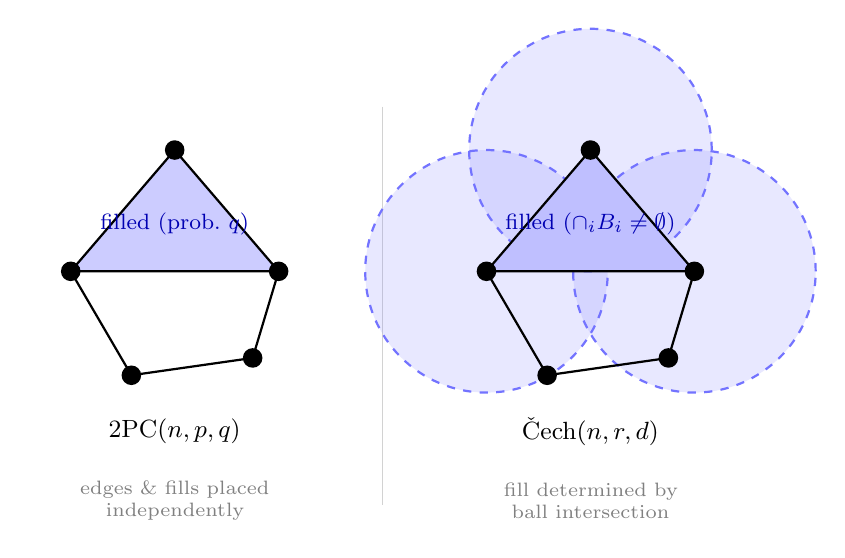
\begin{tikzpicture}[
  vert/.style={circle,fill=black,inner sep=2.5pt},
  scale=1.1
]
%% ─── Left panel: 2PC ────────────────────────────────────────────────────────
\begin{scope}[xshift=0cm]
  \coordinate (A) at ( 0.0,  1.4);
  \coordinate (B) at (-1.2,  0.0);
  \coordinate (C) at ( 1.2,  0.0);
  \coordinate (D) at (-0.5, -1.2);
  \coordinate (E) at ( 0.9, -1.0);
  \fill[blue!20] (A)--(B)--(C)--cycle;
  \draw[thick] (A)--(B) (A)--(C) (B)--(C);
  \draw[thick] (B)--(D) (C)--(E) (D)--(E);
  \foreach \p in {A,B,C,D,E} \node[vert] at (\p) {};
  \node[draw=none,fill=none,font=\footnotesize,blue!70!black] at (0,0.55)
    {filled (prob.\ $q$)};
  \node[draw=none,fill=none,font=\small] at (0,-1.85) {$\PC(n,p,q)$};
  \node[draw=none,fill=none,font=\scriptsize,gray,text width=3.5cm,align=center]
    at (0,-2.65) {edges \& fills placed independently};
\end{scope}
%% ─── Divider ─────────────────────────────────────────────────────────────────
\draw[gray!35,thin] (2.4,1.9)--(2.4,-2.7);
%% ─── Right panel: Čech ───────────────────────────────────────────────────────
\begin{scope}[xshift=4.8cm]
  \coordinate (A2) at ( 0.0,  1.4);
  \coordinate (B2) at (-1.2,  0.0);
  \coordinate (C2) at ( 1.2,  0.0);
  \coordinate (D2) at (-0.5, -1.2);
  \coordinate (E2) at ( 0.9, -1.0);
  \begin{scope}[opacity=0.18]
    \fill[blue!50] (A2) circle (1.4);
    \fill[blue!50] (B2) circle (1.4);
    \fill[blue!50] (C2) circle (1.4);
  \end{scope}
  \draw[blue!55,dashed,thick] (A2) circle (1.4);
  \draw[blue!55,dashed,thick] (B2) circle (1.4);
  \draw[blue!55,dashed,thick] (C2) circle (1.4);
  \fill[blue!25] (A2)--(B2)--(C2)--cycle;
  \draw[thick] (A2)--(B2) (A2)--(C2) (B2)--(C2);
  \draw[thick] (B2)--(D2) (C2)--(E2) (D2)--(E2);
  \foreach \p in {A2,B2,C2,D2,E2} \node[vert] at (\p) {};
  \node[draw=none,fill=none,font=\footnotesize,blue!70!black] at (0,0.55)
    {filled ($\cap_i B_i\neq\emptyset$)};
  \node[draw=none,fill=none,font=\small] at (0,-1.85) {$\Cech(n,r,d)$};
  \node[draw=none,fill=none,font=\scriptsize,gray,text width=3.5cm,align=center]
    at (0,-2.65) {fill determined by ball intersection};
\end{scope}
\end{tikzpicture}
\caption{The two models on $n=5$ vertices (schematic; the paper uses sup-norm balls on
  $\TT^d$). \emph{Left:} Under $\PC(n,p,q)$, each edge appears independently with
  probability~$p$ and each completed triangle is filled independently with probability~$q$
  (shaded); the bottom triangle has all three edges present but no fill.
  \emph{Right:} Under the Rips clique complex $\Cech(n,r,d)$ on $\TT^d$, edges connect
  vertices within distance~$r$ and a triple fills whenever all three pairwise edges are
  present (Helly-2 on the torus ensures the existential nerve agrees with the clique
  condition for the matched-radius regime considered in this paper).}
\label{fig:models}
\end{figure}

\subsection{Parameter Matching}

To compare $\PC$ and $\Cech$ on equal footing, we match the marginal edge probability $p$
and the marginal fill probability $q$.

\begin{definition}[matchRadius]\label{def:matchradius}
Given $p\in(0,1)$ and $d\geq 1$, the \emph{matched radius} is
\begin{equation}\label{eq:matchradius}
  r(p,d) = \frac{p^{1/d}}{2}.
\end{equation}
This is the unique $r\in(0,1/2]$ satisfying $(2r)^d = p$, i.e., the sup-norm ball of radius
$r$ has volume exactly $p$.
\end{definition}

With this choice, points $x_i, x_j$ sampled uniformly on $\TT^d$ satisfy
$\PP[d_\infty(x_i,x_j)\leq r] = p$. The formula~\eqref{eq:matchradius} is formally verified
in Lean as \lean{matchRadius\_spec} \leanverified{matchRadius\_spec}.

\begin{definition}[fillingProb]\label{def:fillingprob}
Let $r = r(p,d)$. The \emph{filling probability} is the marginal probability that the
nerve condition holds on three iid uniform points:
\[
  \fillingP(p,d)
  = \PP\!\left[\bigcap_{\ell=1}^{3} B(x_\ell, r)\neq\emptyset\right],
  \qquad x_1,x_2,x_3\sim_{\mathrm{iid}}\mathrm{Unif}(\TT^d).
\]
\end{definition}

We set $q = \fillingP(p,d)$ so that both models share the same marginal fill probability.
Under this matching, any distributional difference in $\tauf$ reflects geometric dependence,
not marginal mismatch.

We adopt the following vocabulary throughout. A triple $\{i,j,k\}$ is an \emph{empty
triangle} if at least one edge $A_{ij},A_{ik},A_{jk}$ is absent (so $F_{ijk} = 0$
identically under the Rips clique fill~\eqref{eq:fill-clique}); it is a \emph{filled
triangle} if all three edges are present and $F_{ijk} = 1$. Under 2PC, empty and filled
triangles are both random events with conditional probabilities determined by independent
edge and fill draws; under the Rips clique geometric model, the fill is a deterministic
function of the three edge indicators, and all signal in $\geomCov(p,d)$ comes from the
geometric coupling between the three edges via the shared torus positions.

\begin{definition}[geometricCov]\label{def:geomcov}
The \emph{geometric covariance} $\geomCov(p,d)$ is the per-triangle contribution to
$\EE[\tauf]$ under $\Cech(n,r,d)$ with matched parameters:
\begin{equation}\label{eq:geomcov-def}
  \geomCov(p,d)
  = \EE_{\Cech}\!\bigl[(A_{ij}-p)(A_{ik}-p)(A_{jk}-p)(F_{ijk}-q)\bigr],
\end{equation}
where the expectation is over a single triangle $\{i,j,k\}$ drawn uniformly under
$\Cech(n,r,d)$ with $r = r(p,d)$ and $q = \fillingP(p,d)$.
\end{definition}

The quantity $\geomCov(p,d)$ has two distinguishable pieces. The three factors
$(A_e - p)$ form the \emph{BDER signed edge product}: this is the multiplicand that
BDER~\cite{Bubeck2016} use for graph detection on $\Sph^{d-1}$, and it isolates the
pairwise-edge correlations induced by shared latent coordinates. The additional factor
$(F_{ijk} - q)$ is specific to the simplicial setting and centers the fill indicator
relative to its matched marginal. Under the Rips clique fill on $\TT^d$, the regime-free
closed form of Lemma~\ref{lem:radius-asymptotics}(b) determines $\geomCov$ in terms of
$p$ and $q = \fillingP(p,d)$ alone, with the limit $p^3(1-p)^3 > 0$ giving an
$n$-independent positive signal at every dimension. Under proper \v{C}ech fill on the
sphere (\S\ref{sec:sphere-instance}), the existential nerve genuinely strengthens the
clique condition and $\geomCov_{\text{\v{C}ech}}$ vanishes super-exponentially in~$d$,
giving the sub-logarithmic dimensional barrier.

\subsection{Asymptotic Properties of the Matched Parameters}

We record a 1D Helly-type lemma on the circle. This is the structural fact that justifies
identifying the Rips clique fill with the existential nerve on $\TT^d$ in the matched-radius
regime (Remark~\ref{rem:helly2-collapse}); in the present argument the closed form
\lean{geometricCov\_eq} bypasses any explicit appeal to it.

\begin{lemma}[Three-arc intersection]\label{lem:helly}
Let $r \geq 1/3$ and let $x_1,x_2,x_3\in\TT^d$ be arbitrary. Then
$B(x_1,r)\cap B(x_2,r)\cap B(x_3,r)\neq\emptyset$.
\end{lemma}

\begin{proof}
By the product structure $\TT^d = (\AddCircle)^d$, it suffices to prove the statement in
each coordinate separately: three sup-norm balls in $\TT^d$ intersect iff their projections
onto each $\AddCircle$-coordinate intersect. So it suffices to treat the case $d = 1$.

On $\AddCircle = \RR/\ZZ$ with the sup-norm, the ball $B(x_i,r)$ is a closed arc of length
$2r$, and its complement $B(x_i,r)^c$ is an open arc of length $1-2r$.

\textit{Case $r > 1/3$:} The three open complements have lengths $1-2r < 1/3$ each, with
total length $3(1-2r) < 1$. Since they cannot cover $\AddCircle$ (circumference~1), there
exists $y \notin \bigcup_i B(x_i,r)^c$, i.e., $y \in \bigcap_i B(x_i,r)$.

\textit{Case $r = 1/3$:} The three complements have length exactly $1/3$ each. If they do
not cover $\AddCircle$, a common point of the three balls exists as above. If they do cover
$\AddCircle$, they must be pairwise disjoint open arcs forming a partition (up to finitely
many boundary points). Denote the three boundary points (endpoints of the complementary arcs)
by $c_1, c_2, c_3$. Each $c_j$ is an endpoint of exactly two complementary arcs, hence lies
in the closure of two of the balls and in the interior of the third. In particular,
$c_1, c_2, c_3 \in B(x_1, 1/3) \cap B(x_2, 1/3) \cap B(x_3, 1/3)$, so the triple
intersection is nonempty.

In both cases, $\bigcap_i B(x_i, r) \neq \emptyset$.
\end{proof}

With Lemma~\ref{lem:helly} in hand, we turn to the matched parameters.

\begin{lemma}[Radius and covariance asymptotics, Rips clique fill]\label{lem:radius-asymptotics}
Fix $p\in(0,1)$. Under the Rips clique fill~\eqref{eq:fill-clique} on $\TT^d$:
\begin{enumerate}[label=(\alph*)]
\item $r(p,d) = p^{1/d}/2\to 1/2$ as $d\to\infty$; the matched radius increases
  monotonically toward the torus diameter.
  \hfill \leanverified{matchRadius\_tendsto\_half}
\item For all $p \in (0,1)$ and $d \ge 1$,
  $\geomCov(p,d) = q\bigl[(1-p)^3 + p^3\bigr] - q^2$ with $q = \fillingP(p,d)$.
  \hfill \leanverified{geometricCov\_eq}
\item $\geomCov(p,d) \to p^3 (1-p)^3 > 0$ as $d \to \infty$.
  \hfill \leanverified{geometricCov\_tendsto\_pcubed\_compcubed}
\end{enumerate}
In particular, on this Helly-2 ambient there is no $n$-independent dimensional barrier:
$\geomCov$ stabilises at a positive constant.
\end{lemma}

\begin{proof}
\textit{Part~(a).} Since $p\in(0,1)$, we have $\log p < 0$, so
$\log r(p,d) = (\log p)/d - \log 2 \to -\log 2$ as $d\to\infty$, giving $r(p,d)\to 1/2$.
Monotonicity holds because $p^{1/d}$ is increasing in $d$ for $p\in(0,1)$.

\textit{Part~(b).} Expand the doubly-centered product
$\prod_{(e)}(A_e - p)\cdot(F_{ijk} - q)$ with $F_{ijk} = A_{ij} A_{ik} A_{jk}$ and the
matched marginals $\EE[A_e] = p$, $\EE[F_{ijk}] = q$. The mixed-monomial moments
$\EE[\prod A_e^{a_e}]$ reduce, by coordinate factorisation and the edge/wedge
volume identities (\lean{centered\_edge\_moment\_free},
\lean{centered\_edge\_moment\_fill\_free}), to expressions in $p$ and $q$ alone. The
algebraic identity $\geomCov = q[(1-p)^3 + p^3] - q^2$ is the resulting closed form
(regime-free; supersedes the earlier deep-regime expansion of
\lean{geometricCov\_eq\_deep}).

\textit{Part~(c).} The matched marginal $q = \fillingP(p,d) = \PP[\text{three iid}
\text{ points form a }d_\infty\text{-clique of radius }r]$ tends to $p^3$ as
$d \to \infty$ (\lean{fillingProb\_tendsto\_pcubed}): coordinate factorisation gives
$q = \phi(r(p,d))^d$ for the 1D clique probability $\phi(r)$, and the matched edge-pair
probability satisfies $\phi(r(p,d))^d \to p^3$ by independence of the three pairwise
edges in the iid limit. Substituting into part~(b) yields
$p^3[(1-p)^3 + p^3] - p^6 = p^3 (1-p)^3$. \qedhere
\end{proof}

%% ─────────────────────────────────────────────────────────────────────────────
\section{The Doubly-Signed Statistic}\label{sec:statistic}\label{sec:linfty-statistic}
%% ─────────────────────────────────────────────────────────────────────────────

Two natural simplicial analogues of the BDER signed triangle statistic suggest themselves,
and neither is quite right. Centering only the edge indicators (as BDER does for graphs)
gives a statistic sensitive to graph geometry but blind to fill structure; centering only
the fill indicator leaves the edge layer unsigned, so the expectation under $\PC$ picks up
a systematic bias from the correlation between edges and fills. The construction below
centers all four indicators simultaneously: we replace each $A_e$ by $A_e - p$ and
$F_{ijk}$ by $F_{ijk} - q$. This doubly-centered product vanishes in expectation under
$\PC$ (by independence) and isolates the geometric dependence introduced by the
\v{C}ech model.

Let $A_{ij}\in\{0,1\}$ denote the indicator that edge $\{i,j\}$ is present, and let
$F_{ijk}\in\{0,1\}$ denote the indicator that triangle $\{i,j,k\}$ is filled (zero if any
edge is absent). Fix parameters $p,q$ from the null model.

\begin{definition}[Doubly-signed statistic]\label{def:tauf}
The \emph{doubly-signed filled triangle statistic} is
\begin{equation}\label{eq:tauf-def}
  \tauf = \sum_{\{i,j,k\}\in\binom{[n]}{3}}
    \Bigl[\prod_{e\in\partial\{i,j,k\}}(A_e - p)\Bigr](F_{ijk} - q),
\end{equation}
where $\partial\{i,j,k\} = \bigl\{\{i,j\},\{i,k\},\{j,k\}\bigr\}$ denotes the three
boundary edges.
\end{definition}

The factor $\prod_{e\in\partial t}(A_e - p)$ is the BDER signed edge product for
triangle~$t$; the factor $(F_t - q)$ centers the fill indicator. The product is doubly
centered, vanishing in expectation whenever any of the four indicators is independent of the
rest. We write $Z_t = (A_{ij}-p)(A_{ik}-p)(A_{jk}-p)(F_{ijk}-q)$ for the per-triangle
summand, so $\tauf = \sum_t Z_t$.

We first compute the moments under the null model, where full independence reduces the
calculation to products of centered indicators.

\begin{proposition}[Moments under 2PC]\label{prop:moments-twopc}
Under $\PC(n,p,q)$:
\begin{enumerate}[label=(\alph*)]
\item $\EE[\tauf] = 0$.
\item $\Var[\tauf] = \binom{n}{3}\cdot p^3(1-p)^3\cdot q(1-q)$.
  In particular, $\Var[\tauf\mid\PC] = \Theta(n^3)$.
\end{enumerate}
\hfill \leanverified{moments\_twoParam\_signed}
\end{proposition}

\begin{proof}
\textit{Part~(a).} Under $\PC$, all four indicators $A_{ij}, A_{ik}, A_{jk}, F_{ijk}$ are
mutually independent. Hence
\[
  \EE[Z_t] = \EE[A_{ij}-p]\cdot\EE[A_{ik}-p]\cdot\EE[A_{jk}-p]\cdot\EE[F_{ijk}-q] = 0,
\]
since $\EE[A_{ij}-p] = 0$. Summing over all $\binom{n}{3}$ triangles gives $\EE[\tauf]=0$.

\textit{Part~(b), off-diagonal terms.} For distinct triangles $t\neq t'$, we show
$\EE[Z_t Z_{t'}] = 0$. Under $\PC$, all edge and fill indicators are mutually independent.
Any edge $e \in \partial t \setminus \partial t'$ that appears in $t$ but not $t'$ contributes
an independent factor $(A_e - p)$ to $Z_t$ which is independent of $Z_{t'}$; since
$\EE[A_e-p]=0$, the product $\EE[Z_t Z_{t'}]=0$. The same argument applies if $t,t'$
share all three edges (impossible for distinct triangles) or if the fill $F_t$ is unshared.
More precisely: whenever any indicator in the product $Z_t Z_{t'}$ appears in exactly one of
$Z_t, Z_{t'}$, it contributes a mean-zero factor independent of the rest, killing the
expectation. One checks case by case that for any two distinct triangles (sharing 0, 1, 2, or
3 vertices), at least one such unshared indicator exists.

\textit{Part~(b), diagonal terms.} By mutual independence in $\PC$,
\begin{align*}
  \Var[Z_t] = \EE[Z_t^2]
  &= \EE[(A_{ij}-p)^2]\cdot\EE[(A_{ik}-p)^2]\cdot\EE[(A_{jk}-p)^2]\cdot\EE[(F_{ijk}-q)^2]\\
  &= p(1-p)\cdot p(1-p)\cdot p(1-p)\cdot q(1-q).
\end{align*}
Since the $\binom{n}{3}$ diagonal terms are uncorrelated, summing gives
$\Var[\tauf] = \binom{n}{3}\cdot p^3(1-p)^3 q(1-q)$.
\end{proof}

Under the \v{C}ech model the three vertices of a triangle are coupled through their
shared positions on $\TT^d$, and covariance across triangles is nontrivial only when
two triangles share an edge.

\begin{proposition}[Moments under \v{C}ech]\label{prop:moments-cech}
Under $\Cech(n,r,d)$ with $r = r(p,d)$ and matched $q = \fillingP(p,d)$:
\begin{enumerate}[label=(\alph*)]
\item $\EE[\tauf] = \binom{n}{3}\cdot\geomCov(p,d)$.
  \hfill \leanverified{moments\_cech\_signed}
\item $\Var[\tauf] = O(n^4)$.
  \textup{(Pen-and-paper; see Appendix~\ref{app:variance-bound}.)}
\end{enumerate}
\end{proposition}

\begin{proof}
\textit{Part~(a).}
Write $Z_t = (A_{ij}-p)(A_{ik}-p)(A_{jk}-p)(F_{ijk}-q)$ for triangle $t = \{i,j,k\}$.
Under the \v{C}ech model, the joint law of $(A_{ij}, A_{ik}, A_{jk}, F_t)$ is determined by
the triple $(x_i,x_j,x_k)$ drawn uniformly on $(\TT^d)^3$. By definition of
$\geomCov(p,d)$~\eqref{eq:geomcov-def}, we have $\EE[Z_t] = \geomCov(p,d)$ for each
triangle. Since all $\binom{n}{3}$ triangles are identically distributed,
$\EE[\tauf] = \binom{n}{3}\cdot\geomCov(p,d)$.

\textit{Part~(b).}
Expand $\Var[\tauf] = \sum_{t,t'} \Cov(Z_t, Z_{t'})$ and classify pairs $(t,t')$ by the number
$s\in\{0,1,2,3\}$ of shared vertices ($s=3$ corresponds to the diagonal $t=t'$). The
contribution from each class is summarized by the following counts:
\begin{center}
\renewcommand{\arraystretch}{1.1}
\begin{tabular}{c|c|c|c}
shared vertices $s$ & $\#\{(t,t')\}$ & $\Cov(Z_t, Z_{t'})$ per pair & total \\
\hline
$s=3$ (diagonal) & $\binom{n}{3} = \Theta(n^3)$ & $\leq\Var[Z_t]\leq 1$ & $O(n^3)$ \\
$s=2$ (shared edge) & $\binom{n}{2}(n-2)(n-3) = \Theta(n^4)$ & $O(1)$ & $O(n^4)$ \\
$s=1$ (shared vertex) & $n\binom{n-1}{2}\binom{n-3}{2} = \Theta(n^5)$ & $0$ & $0$ \\
$s=0$ (disjoint) & $\binom{n}{3}\binom{n-3}{3} = \Theta(n^6)$ & $0$ & $0$ \\
\end{tabular}
\end{center}

Since $|Z_t|\leq 1$ by construction, all per-pair covariances are bounded by $O(1)$. The
$s=0$ case is immediate from the independence of the six distinct sampled points. The $s=1$
and $s=2$ cases require the conditioning arguments sketched below; the full derivation is
given in Appendix~\ref{app:variance-bound}.

\smallskip
\noindent\emph{Case $s=1$ (zero contribution).} Suppose $t=\{i,j,k\}$ and $t'=\{i,j',k'\}$
share only the vertex~$i$. Condition on $x_i$ and apply the law of total covariance:
\[
  \Cov(Z_t,Z_{t'}) \;=\; \underbrace{\EE\!\bigl[\Cov(Z_t,Z_{t'}\mid x_i)\bigr]}_{\text{first term}}
  \;+\; \underbrace{\Cov\!\bigl(\EE[Z_t\mid x_i],\EE[Z_{t'}\mid x_i]\bigr)}_{\text{second term}}.
\]
The first term vanishes by \emph{conditional independence}: given $x_i$, the points
$(x_j,x_k)$ are independent of $(x_{j'},x_{k'})$ (four independent uniform draws on $\TT^d$),
so $Z_t$ and $Z_{t'}$ are conditionally independent and their conditional covariance is $0$.
The second term vanishes by \emph{translation invariance}: under the uniform measure on
$\TT^d$, the law of $(x_j - x_i, x_k - x_i)\pmod 1$ is uniform on $(\TT^d)^2$ regardless
of the value of $x_i$. Hence the conditional law of $Z_t$ given $x_i$ does not depend on
$x_i$; in particular $\EE[Z_t\mid x_i] = \EE[Z_t]$ is a constant, and symmetrically for $t'$.
A covariance of two constants is zero.

\smallskip
\noindent\emph{Case $s=2$ (the only nontrivial contribution, $O(n^4)$).} For triangles
$t=\{i,j,k\}$ and $t'=\{i,j,k'\}$ sharing edge $\{i,j\}$, condition on $(x_i,x_j)$; the
remaining points $x_k, x_{k'}$ are then conditionally iid uniform on $\TT^d$, so $Z_t$ and
$Z_{t'}$ become conditionally independent functions of $(x_i,x_j)$. The Cauchy--Schwarz-type
bound $|\Cov(Z_t,Z_{t'})|\leq 1$ combines with the count $\Theta(n^4)$ to give the leading
$O(n^4)$ term.

Combining the four cases yields $\Var[\tauf] = O(n^3)+O(n^4)+0+0 = O(n^4)$.
\end{proof}

%% ─────────────────────────────────────────────────────────────────────────────
\section{Paper~1: Detection on the $\ell^\infty$ Torus (Helly-2)}\label{sec:linfty-detection}\label{sec:detection}
%% ─────────────────────────────────────────────────────────────────────────────

Throughout this section, $\TV(\mu,\nu) = \sup_{A}|\mu(A) - \nu(A)|$ denotes the total
variation distance between probability measures $\mu$ and $\nu$.

\begin{lemma}[Signal-to-noise bound]\label{lem:snr}
With matched parameters $r = r(p,d)$ and $q = \fillingP(p,d)$,
\begin{equation}\label{eq:snr}
  \mathrm{SNR}(\tauf)
  \;=\; \frac{\bigl(\EE_{\Cech}[\tauf]-\EE_{\PC}[\tauf]\bigr)^2}{\Var_{\PC}[\tauf]}
  \;=\; \binom{n}{3}\cdot\frac{\geomCov(p,d)^2}{p^3(1-p)^3 q(1-q)}.
\end{equation}
In particular, $\mathrm{SNR}\to\infty$ if and only if
\begin{equation}\label{eq:detection-cond}
  n^{3/2}\cdot\geomCov(p,d)\to\infty.
\end{equation}
\end{lemma}

\begin{proof}
By Propositions~\ref{prop:moments-twopc}(a) and~\ref{prop:moments-cech}(a),
$\EE_{\Cech}[\tauf]-\EE_{\PC}[\tauf] = \binom{n}{3}\geomCov(p,d)$ and
$\Var_{\PC}[\tauf] = \binom{n}{3}p^3(1-p)^3 q(1-q)$. Substituting gives~\eqref{eq:snr}.
Since $\binom{n}{3}=\Theta(n^3)$, $\mathrm{SNR}\to\infty$ iff $n^3\geomCov(p,d)^2\to\infty$,
i.e.,~\eqref{eq:detection-cond}.
\end{proof}

\subsection{The Detection Theorem}

\begin{theorem}[Detection lower bound]\label{thm:detection}
Fix $p\in(0,1)$, fix $d$ with $\geomCov(p,d) > 0$, and let $q = \fillingP(p,d)$. Then
the test that rejects~$\PC$ when $\tauf$ exceeds a suitable threshold achieves asymptotic
power~$1$ as $n\to\infty$:
\[
  \TV\bigl(\PC(n,p,q),\,\Cech(n,r(p,d),d)\bigr)\to 1.
\]
\hfill \leanverified{detection\_lower\_bound\_fixed\_d}
\end{theorem}

\begin{proof}
Let $g = \geomCov(p,d) > 0$ by hypothesis, and let $\mu_C = \EE_{\Cech}[\tauf] = \binom{n}{3}g$.
Since $d$ is fixed, $g$ is a positive constant independent of $n$.
Set the threshold at $\theta = \mu_C/2$.

\textit{2PC side: probability above threshold goes to~0.}
By Chebyshev's inequality and Proposition~\ref{prop:moments-twopc},
\[
  \PP_{\PC}\!\left[\tauf > \theta\right]
  \;\leq\; \PP_{\PC}\!\left[|\tauf| > \theta\right]
  \;\leq\; \frac{\Var_{\PC}[\tauf]}{\theta^2}
  = \frac{\binom{n}{3}p^3(1-p)^3 q(1-q)}{\bigl(\frac{1}{2}\binom{n}{3}g\bigr)^2}
  = \frac{4p^3(1-p)^3 q(1-q)}{\binom{n}{3}g^2}.
\]
Since $d$ is fixed, $g>0$ is a positive constant, so $\binom{n}{3}g^2 = \Omega(n^3)\to\infty$.
Therefore $\PP_{\PC}[\tauf > \theta] \to 0$.
\hfill \leanverified{chebyshev\_2PC\_prob\_tendsto\_zero}

\textit{\v{C}ech side: probability above threshold goes to~1.}
We apply the Paley--Zygmund inequality: for any nonnegative random variable $W$,
$\PP[W > 0] \geq (\EE W)^2/\EE[W^2]$. Apply this with $W = (\tauf - \theta)_+$, using
that $\tauf \geq \theta$ implies $W = \tauf - \theta \geq 0$. More directly, the
Paley--Zygmund inequality gives
\[
  \PP_{\Cech}\!\left[\tauf > \tfrac{1}{2}\mu_C\right]
  \geq \frac{1}{4}\cdot\frac{\mu_C^2}{\EE_{\Cech}[\tauf^2]}.
\]
The numerator is $\mu_C^2 = \binom{n}{3}^2 g^2 = \Omega(n^6 g^2)$. For the denominator,
$\EE_{\Cech}[\tauf^2] = (\EE_{\Cech}[\tauf])^2 + \Var_{\Cech}[\tauf] \leq \mu_C^2 + Cn^4$
by Proposition~\ref{prop:moments-cech}(b). Therefore
\[
  \PP_{\Cech}\!\left[\tauf > \tfrac{1}{2}\mu_C\right]
  \geq \frac{c\,n^6 g^2}{n^6 g^2 + C n^4}
  = \frac{c}{1 + C/(n^2 g^2)}.
\]
Since $d$ is fixed and $g>0$ is a positive constant, $n^2g^2\to\infty$, giving the
denominator $\to 1$ and the lower bound $\to c > 0$. A more careful estimate shows the
bound tends to~1: rewrite as $1 - Cn^4/(n^6g^2+Cn^4) = 1 - o(1)$ since $n^2g^2\to\infty$.
\hfill \leanverified{paleyZygmund\_cech\_prob\_tendsto\_one}

Since $\PP_{\PC}[\tauf > \theta]\to 0$ and $\PP_{\Cech}[\tauf > \theta]\to 1$ for the same
threshold, the two pushforward distributions
$\mathrm{law}_{\PC}(\tauf)$ and $\mathrm{law}_{\Cech}(\tauf)$ (each a probability measure
on $\RR$ obtained by applying the real-valued statistic $\tauf$ to the corresponding
random complex) separate to $\TV = 1$ on the event $\{\tauf > \theta\}$. The
data-processing inequality for total variation---applying a measurable function cannot
increase $\TV$---then gives
$\TV(\PC,\Cech) \geq \TV(\mathrm{law}_{\PC}(\tauf), \mathrm{law}_{\Cech}(\tauf))\to 1$, so
$\TV(\PC,\Cech)\to 1$.
\end{proof}

\subsection{No-Barrier Regime: Joint $(n,d)$ Detection}

Theorem~\ref{thm:detection} combined with Lemma~\ref{lem:radius-asymptotics}(c) gives
the headline conclusion: on the $\ell^\infty$ torus with Rips clique fill, there is
\emph{no $n$-independent dimensional barrier}. For every fixed $p \in (0,1)$ and every
fixed $d \ge 1$, $\geomCov(p, d) > 0$ (Lemma~\ref{lem:radius-asymptotics}(b,c)), so the
hypothesis of Theorem~\ref{thm:detection} is automatically satisfied and TV $\to 1$ as
$n \to \infty$. The joint-$(n,d)$ strengthening below gives the corresponding statement
when $d$ is also allowed to grow.

\begin{theorem}[Joint $(n, d)$ detection]\label{thm:phase-transition}
Fix $p \in (0, 1)$. Suppose $\geomCov(p, d) \sim G \cdot d^{-\alpha}$ as $d \to \infty$
for some constants $G > 0$ and $\alpha > 0$ (i.e.\
$\geomCov(p, d) / (G \cdot d^{-\alpha}) \to 1$). Let $n_k \to \infty$ and $d_k \to \infty$
be integer sequences with $d_k / (n_k G)^{1/\alpha} \to 0$. Then with
$q_k = \fillingP(p, d_k)$,
\[
  \TV\!\bigl(\PC(n_k, p, q_k),\;
    \Cech(n_k, r(p, d_k), d_k)\bigr) \to 1.
\]
\hfill \leanverified{phase\_transition}
\end{theorem}

\begin{remark}[Scope of the no-barrier conclusion]\label{rem:tv-zero-caveat}
The headline ``no $n$-independent dimensional barrier'' is a statement about the
doubly-signed statistic $\tauf$ on the Rips clique fill: detection succeeds via $\tauf$ at
every fixed $d \ge 1$. It does not preclude lower-bound results in extreme scaling regimes
or for richer test statistics; we leave matching impossibility bounds open. The sphere
instance (\S\ref{sec:sphere-instance}) gives a structurally different setting where a
genuine $d$-dependent barrier emerges via the Helly-$d$ structure of $S^{d-1}$.
\end{remark}

%% ─────────────────────────────────────────────────────────────────────────────
\section{Discussion}\label{sec:discussion}
%% ─────────────────────────────────────────────────────────────────────────────

\subsection{Comparison with BDER}\label{sec:comparison-bder}

The connection to Bubeck, Ding, Eldan, and R\'acz~\cite{Bubeck2016} is the organizing
principle of this work. BDER established that the signed triangle statistic
$\tau_\Delta = \sum_t\prod_{e\in\partial t}(A_e - p)$ detects latent $d$-dimensional
geometry in a random graph on $\Sph^{d-1}$ when $d \ll n^3$ and fails when
$d\gg n^3$. Their detection is driven by the BDER pairwise covariance
$\mathrm{cov}_{ij,ik}(d)\sim C/\sqrt{d}$, positive for every finite $d$; the
threshold $d^*_{\mathrm{BDER}}\asymp n^3$ is therefore set by the SNR condition
$n^3\,\mathrm{cov}^2\to\infty$ and \emph{grows with}~$n$.

Our $\tauf$ adds a second layer of centering for the fill indicator, and $\geomCov(p,d)$
plays the role of $\mathrm{cov}_{ij,ik}$ in the detection condition
$n^{3/2}\cdot\geomCov(p,d)\to\infty$ (Lemma~\ref{lem:snr}). On $\TT^d$ with Rips clique
fill, the Helly-2 structure of the ambient ensures $\geomCov \to p^3(1-p)^3 > 0$ at fixed
$p$ (Lemma~\ref{lem:radius-asymptotics}(c)), so the detection regime is qualitatively
BDER-like: signal is preserved at every finite $d$ and the SNR condition determines
the joint $(n, d)$ threshold (Theorem~\ref{thm:phase-transition}). The Helly-$d$ sphere
instance of \S\ref{sec:sphere-instance} is genuinely different: there the existential
\v{C}ech nerve cannot be collapsed onto the clique, and a sub-logarithmic dimensional
barrier emerges.

A direct expansion of $\geomCov(p,d)$, using $q = \EE_{\Cech}[F_{ijk}]$, gives the
covariance identity
\begin{equation}\label{eq:geomcov-as-covariance}
  \geomCov(p,d) \;=\; \mathrm{Cov}_{\Cech}\!\bigl(\textstyle\prod_{e\in\partial t}(A_e - p),\, F_{ijk}\bigr).
\end{equation}
That is, our per-triangle signal is exactly the covariance between BDER's signed edge
product and the fill indicator. Under the Rips clique fill on $\TT^d$, $F_{ijk}$ is a
function of the three edge indicators, so this covariance reduces to the closed form of
Lemma~\ref{lem:radius-asymptotics}(b); the relative magnitude vs.\ the BDER signed edge
product is set by the difference $q[(1-p)^3 + p^3] - q^2$ vs.\ the matched edge moment.

\subsection{Quantitative deep-regime expansion and the sparse regime}\label{sec:quantitative}

The 1D primitive $\phi(r) = \PP[\text{three iid arcs of length }2r\text{ on }\TT^1\text{ pairwise
agree}]$ admits the closed form $\phi(r) = 12 r^2$ for $r \in [0, 1/4]$ via
Stevens~\cite{Stevens1939}, and by coordinate factorisation
$\fillingP(p, d) = \phi(r(p, d))^d$ in the deep regime $r \le 1/4$.
Expanding $\geomCov$ into monomials and applying the wedge--fill identity
\lean{wedge\_implies\_fill} yields the deep-regime expansion
\begin{equation}\label{eq:geomcov-deep}
  \geomCov(p,d) = (1-q)\,(3r^2)^d + 3p^3\bigl[(7r/2)^d - 1\bigr], \qquad r \leq 1/4,
\end{equation}
verified in Lean as \lean{geometricCov\_eq\_deep}. The regime-free identity of
Lemma~\ref{lem:radius-asymptotics}(b) (\lean{geometricCov\_eq}) supersedes this expansion
in the sense of dropping the $r \le 1/4$ hypothesis; the deep-regime form remains useful
because it exposes the explicit $(3r^2)^d$ and $(7r/2)^d$ factors that drive the
sparse-regime detection corollary below.

Combining~\eqref{eq:geomcov-deep} with the $n^{3/2}$ Paley--Zygmund SNR condition of
Theorem~\ref{thm:detection} yields a clean sparse-regime corollary.

\begin{corollary}[Sparse-regime detection]\label{cor:sparse}
Let $(p_n, d_n)_{n\geq 1}$ satisfy $r(p_n,d_n) \leq 1/4$, $p_n \to 0$, and
\begin{equation}\label{eq:sparse-snr}
  n^{3/2} \cdot (3/4)^{d_n} \cdot p_n^2 \to \infty.
\end{equation}
Then $\tauf$ achieves asymptotic power $1$: $\TV(\PC(n,p_n,q_n),\Cech(n,r(p_n,d_n),d_n))\to 1$.
\end{corollary}

\noindent
\emph{Fixed dimension.} For $d$ fixed and $p_n = n^{-\alpha}$, condition~\eqref{eq:sparse-snr}
reduces to $\alpha < 3/4$, giving the sparse threshold $p_n \gg n^{-3/4}$. This is the simplicial
analogue of the sparse RGG threshold of Liu--Mohanty--Schramm--Yang~\cite{Liu2022} for graphs on
$\Sph^{d-1}$.

\emph{Joint $(n,d,p)$ scaling.} Detection is possible when
$d_n\log(4/3) + 2|\!\log p_n| \ll (3/2)\log n$, opening a three-dimensional detectable region
in $(n,d,p)$-space.

\subsection{The fill-pair statistic}\label{sec:fillfill}

In the graph detection problem on $\Sph^{d-1}$, the signed triangle statistic is optimal among
low-degree polynomial tests (Bangachev--Bresler~\cite{BangachevBresler2024}). The simplicial
setting exhibits a qualitatively different behaviour: a \emph{pure-fill pair} statistic achieves
strictly higher SNR than $\tauf$ throughout the deep regime.

Define the \emph{fill-pair statistic}
\[
  \tauff := \sum_{\substack{t,\, t' \in \binom{[n]}{3} \\ |t \cap t'| = 2}}
            (F_t - q)(F_{t'} - q),
\]
which sums over pairs of triangles sharing exactly one edge. This is a degree-$2$ polynomial
in the fill indicators $\{F_t\}$ and uses no edge information.

\begin{proposition}[Fill-pair SNR]\label{prop:fillfill}
In the deep regime $r(p,d) \leq 1/4$:
\begin{align}
  \EE_{\Cech}[\tauff] &= \tbinom{n}{2}\tbinom{n-2}{2} \cdot
    \bigl[(112r^3/3)^d - (12r^2)^{2d}\bigr], \label{eq:tauff-mean}\\
  \Var_{2\mathrm{PC}}[\tauff] &= \tbinom{n}{2}\tbinom{n-2}{2} \cdot (q(1-q))^2,
    \label{eq:tauff-var}
\end{align}
where $(112r^3/3)^d - (12r^2)^{2d}$ is the covariance between fills of two adjacent triangles
under the \v{C}ech model. The ratio
\[
  \frac{\mathrm{SNR}(\tauff)}{\mathrm{SNR}(\tauf)}
  \approx \sqrt{\tfrac{3n}{2}} \cdot (12.9)^{d/2} \cdot p^{3/2}
\]
grows without bound as $d \to \infty$ for fixed $n,p$.
\end{proposition}

\textbf{Implication.} $\tauf$ detects simplicial structure via joint edge-fill correlation;
$\tauff$ exploits purely the fill-fill covariance between adjacent triangles. The latter signal
is absent in the graph setting (there are no fill bits), which is why the optimality result
of~\cite{BangachevBresler2024} does not transfer. Numerically at $(n,p,d) = (1000,0.01,3)$:
$\mathrm{SNR}(\tauff)/\mathrm{SNR}(\tauf) \approx 1.64$; at $d = 5$ the ratio is $\approx 23$.

\textbf{Lean status.} The key integral $(112r^3/3)^d = \EE_{\Cech}[F_t \cdot F_{t'}]$ for adjacent
$t,t'$ is formally verified in Lean~4 (\texttt{doubleFill\_joint\_prob}, May~2026) via Fubini
and coordinate factorisation over the $d$ torus components. The combinatorial
identities~\eqref{eq:tauff-mean}--\eqref{eq:tauff-var} follow from independence of non-adjacent
fill pairs under 2PC and Fubini conditioning for the \v{C}ech mean.

Whether $\tauff$ is itself low-degree optimal, or whether an even higher-degree polynomial achieves
better SNR, remains open.

\subsection{Limitations}

Paper~1 is restricted to the flat torus $\TT^d$ with the sup-norm metric, where the
ball-volume formula $(2r)^d$ yields the explicit matched radius $r(p,d) = p^{1/d}/2$ and
the Helly-2 structure collapses the existential nerve onto the Rips clique. The detection
conclusion is a positive statement about $\tauf$ and not a matching lower bound on
complex-level indistinguishability; lower bounds for $\TV(\PC, \Cech)$ in restricted
scaling regimes are left open (Remark~\ref{rem:tv-zero-caveat}).

Paper~2 (sphere instance) requires concentration of measure on $S^{d-1}$ with proper
\v{C}ech fill, and currently reduces to six explicitly named structural axioms in
\texttt{Geometry/Sphere.lean}; replacing these with full Mathlib-derived proofs is
ongoing.

\subsection{Open Problems}\label{sec:open}

\subsubsection*{Two-sided rate for $\geomCov$ in sub-regimes}
The closed form~\eqref{eq:geomcov-deep} gives the upper bound
$\geomCov \leq (1-q)(3r^2)^d + 3p^3(7r/2)^d$. The matching lower bound
$\geomCov \geq c(1-q)(3r^2)^d$ holds when $(1-q)(3r^2)^d \gtrsim p^3(7r/2)^d$,
i.e.\ when $1-q \gtrsim p\cdot(7/(6r))^d$. This is \emph{not} uniform across the
deep regime: as $r\to 0$ the lower-bound threshold tightens. Identifying the exact
sub-regime in which the rate is $\Theta$, not just $O$, is open.

\subsubsection*{Higher-dimensional simplices}
The construction generalizes to $k$-simplices for $k\geq 2$ via a multiply-signed
statistic
\(
  \tau_{(k)} = \sum_{\sigma\in\binom{[n]}{k+1}}
    \bigl[\prod_{e\in\partial^{(1)}\sigma}(A_e - p)\bigr](F_\sigma - q_k)
\)
centering all $\binom{k+1}{2}$ boundary edges together with the $k$-face fill
$F_\sigma$. Under the Rips clique fill $F_\sigma = \prod_e A_e$, the moment chain and
no-barrier analysis are expected to carry over with $\Var[\tau_{(k)} \mid (k{+}1)\PC]
= \binom{n}{k+1} \cdot p^{\binom{k+1}{2}}(1-p)^{\binom{k+1}{2}}\, q_k(1-q_k)$ and SNR
exponent $(k+1)/2$. The corresponding sphere instance with proper $k$-face \v{C}ech fill
should give a sub-logarithmic dimensional barrier of the form
$d^*_k(n, p) = (\binom{k+1}{2}\!/\!1) \log n / \log\log n$ via a $k$-dimensional Wishart
extension of Appendix~\ref{app:wishart}. Both generalisations are left open.

\subsubsection*{Low-degree optimality}
As shown in \S\ref{sec:fillfill}, $\tauf$ is \emph{not} low-degree optimal: the fill-pair
statistic $\tauff$ achieves strictly higher SNR throughout the deep regime. Whether $\tauff$
is itself optimal among degree-$\leq D$ polynomials in $(A,F)$---or whether higher-degree
combinations dominate---remains open. The low-degree frameworks of
Bangachev--Bresler~\cite{BangachevBresler2024}, Yu--Zadik--Zhang~\cite{Yu2024},
and Dhawan--Mao--Wein~\cite{DhawanMaoWein2023} provide tools; cataloguing all
degree-$\leq D$ Fourier contributions to the \v{C}ech--$2\PC$ likelihood ratio is the
natural next step.

\subsubsection*{Beyond the flat torus}
Porting the analysis to the sphere $\Sph^{d-1}$ with geodesic distance replaces the
Helly argument with spherical-cap intersections and a transcendental matched-radius
formula. The sphere companion section (\S\ref{sec:sphere-instance}, formerly a planned
separate paper) develops this in detail: under
proper \v{C}ech complex definition on $\Sph^{d-1}$ (Helly number $d$), concentration
of measure forces caps to nearly hemispheres at matched fixed $p$, but the existential
\v{C}ech fill saturates ($q_{\text{\v{C}ech}} \to 1$) while Rips fill collapses
($q_{\text{Rips}} \to p^3$). The covariance signal vanishes super-exponentially:
$1 - q_{\text{\v{C}ech}}(p,d) \sim (3 z_p^2/d)^{(d-2)/2}$ where $z_p = \Phi^{-1}(1-p)$,
driven by the singularity of the joint Gram-entry density
$\propto (\det G)^{(d-4)/2}$ at the boundary $\det G = 0$. Detection threshold:
$d^*(n,p) = 3 \log n / \log\log n$, sub-logarithmic.

\textbf{Note (revised May 2026).} An earlier draft hypothesized that the $L^2$ Euclidean
torus (Helly number $d{+}1$) would give an intermediate detection threshold $\Theta(\log n)$
between the $\ell^\infty$ no-barrier and the sphere $\Theta(\log n / \log\log n)$ result.
\S\ref{sec:lp-nogo} shows this expectation is incorrect: on any \emph{centered}
ambient with iid coordinates (Gaussian, uniform, Bernoulli; under any $\ell^p$ metric
for $p \in [1,\infty)$), the matched radius $r_d$ eventually exceeds the typical
distance from samples to the origin, so the origin becomes a free \v{C}ech witness for
every triple and the dimensional-barrier story \emph{trivialises}. The sphere construction
is essentially canonical: it escapes trivialisation only by having no interior reference
point. Extensions to other latent geometries e.g.\ anisotropic~\cite{Brennan2022}
or hyperbolic~\cite{Litvak2022}, where triangle-based tests behave differently,
remain open.

%% ─────────────────────────────────────────────────────────────────────────────
\section{Sister Instances: A Unified Three-Instance Framework}\label{sec:sister-instances}
%% ─────────────────────────────────────────────────────────────────────────────

The detection problem of \S\ref{sec:intro} is parameterized by the choice of latent
ambient $(\Omega, d_\Omega)$ and complex type (\v{C}ech vs.\ Rips). Three natural
choices give qualitatively different detection landscapes, unified by the Helly
number of the ambient space.

\subsection{Instance 1: $\ell^\infty$ torus / Rips (this paper)}\label{sec:linfty-instance}

The main subject of this paper. Helly number $2$ (1D Helly lemma on the circle).
Detection theorem~\ref{thm:detection} succeeds for every $d \ge 1$ at fixed $p$;
$\geomCov(p,d) \to p^3(1-p)^3 > 0$. \emph{No dimensional barrier.}

\subsection{Instance 2: Sphere $S^{d-1}$ / \v{C}ech (sphere instance)}\label{sec:sphere-instance}

Helly number $d$ (Helly's theorem on $\Sph^{d-1}$ with spherical caps). At fixed $p$,
the matched cosine threshold $r_d = \cos\theta_d$ satisfies $\sqrt{d} \cdot r_d \to \Phi^{-1}(1-p)$
by CLT on cap probability (Lean: \texttt{matchedCos\_asymptotic}, sphere instance
file \texttt{Geometry/Sphere.lean}). The Rips clique probability $q_{\text{Rips}}(p,d) \to p^3$,
while \v{C}ech triple-cover saturates: $q_{\text{\v{C}ech}}(p,d) \to 1$
super-exponentially with tail $1 - q_{\text{\v{C}ech}}(p,d) \sim (3 z_p^2 / d)^{(d-2)/2}$,
driven by the joint Gram-entry density $\propto (\det G)^{(d-4)/2}$ singularity at
$\det G = 0$ (Wishart-derived; full derivation in Appendix~\ref{app:wishart}). Headline:
\[
  \geomCov_{\text{\v{C}ech}}(p,d) \sim p^3 \cdot (3 z_p^2 / d)^{(d-2)/2}
\]
giving a sub-logarithmic detection threshold $d^*(n,p) = 3 \log n / \log\log n$.

The Lean catalog for this instance is in \texttt{SimplicialLatentGeometry/Geometry/Sphere.lean}.
As of May~2026 (post-session-77 follow-up, branch \texttt{oq-18-rips}) the file declares
exactly \textbf{6 named structural axioms}, all documented inline with their mathematical
content:
\begin{itemize}[leftmargin=*, itemsep=2pt]
  \item \texttt{capProb\_continuous} --- continuity of the
    spherical-cap probability $\Pr_{x \sim \mathrm{Unif}(S^{d-1})}[\langle e_0, x\rangle \ge r]$
    in the threshold $r$. The endpoint values $\mathrm{capProb}\,d\,(-1) = 1$ and
    $\mathrm{capProb}\,d\,1 = 0$ are now theorems (commits \texttt{391ef9c} and
    \texttt{29bfcdf}, May~2026), reducing the axiom count from 8 to~6.
  \item \texttt{matchedCos\_exists} --- existence of $r \in [-1, 1]$ with
    $\mathrm{capProb}\,d\,r = p$ (IVT instance, deferred).
  \item \texttt{normalQuantile} --- the standard-normal quantile constant
    $\Phi^{-1}$, used as an opaque value pending Mathlib coverage.
  \item \texttt{capCLT\_matched\_inversion} --- uniform CLT inversion: any
    sequence $r_d$ with $\mathrm{capProb}\,d\,r_d = p$ satisfies
    $\sqrt d \cdot r_d \to \Phi^{-1}(1 - p)$ (Poincaré / Li 2011 limit, deferred).
  \item \texttt{cechFillProb\_compl\_le\_gram\_tail} --- the Wishart Gram-density
    tail bound $1 - q_{\text{\v{C}ech}}(p,d) \le \bigl(3 z_p^2 / d\bigr)^{(d-2)/2}$
    eventually (Paper~2 structural; see Appendix~\ref{app:wishart}).
  \item \texttt{geomCovCech\_decomp\_ratio\_tendsto} --- the algebraic
    decomposition ratio
    $\geomCov_{\text{\v{C}ech}}(p,d) / \bigl(p^3 (1 - q_{\text{\v{C}ech}}(p,d))\bigr) \to 1$
    (Paper~2 structural; see Appendix~\ref{app:wishart}).
\end{itemize}
The asymptotic headlines \texttt{cechFillProb\_tail\_asymptotic} and
\texttt{geomCovCech\_asymptotic} are \emph{derived} from these six axioms via
a pure analytic squeeze (\texttt{gram\_tail\_bound\_tendsto\_zero}). The axiom
count dropped from 17 (session~70) through 12 (session~77, commits
\texttt{b63fc28} concretising \texttt{uniformOnSphere} via
\texttt{Measure.toSphere} and \texttt{51fa5ff} concretising
\texttt{cechFillProb}/\texttt{ripsFillProb}/\texttt{geomCovCech} as iid
product-measure integrals), to 8 (commits \texttt{1b1c739} promoting
\texttt{cechFillProb\_le\_one} to a theorem and \texttt{66ae0c5} closing
\texttt{capProb\_mem\_unitInterval} and \texttt{capProb\_antitone}), and finally to the
current 6 (commits \texttt{391ef9c} and \texttt{29bfcdf} promoting
\texttt{capProb\_neg\_one} and \texttt{capProb\_one} from axioms to theorems,
May~2026).

\subsection{Instance 3: $L^2$ and $\ell^p$ Euclidean ambients (no-go)}\label{sec:lp-nogo}

For any centered iid-coord ambient on $\mathbb R^d$ with finite moments, under any
$\ell^p$ metric with $p \in [1, \infty)$, the fixed-$p$ matched radius eventually exceeds
the typical sample-to-origin distance, and the dimensional-barrier story trivialises.

\begin{proposition}[$\ell^p$ centered-ambient trivialisation]\label{prop:lp-nogo}
  Let $X \in \mathbb R$ be a non-degenerate symmetric random variable with
  $\mu_p := \mathbb E[|X|^p] < \infty$ and
  $\tilde\mu_p := \mathbb E[|X_1 - X_2|^p] < \infty$
  for some $p \ge 1$, where $X_1, X_2$ are iid copies of $X$. Let
  $x_1, \dots, x_n \in \mathbb R^d$ be iid with iid coordinates from $X$, and let $r_d$
  satisfy $\Pr[\|x_1 - x_2\|_p \le r_d] = p_{\mathrm{edge}}$ for fixed $p_{\mathrm{edge}} \in (0,1)$.
  Then there exists $d_0$ such that for all $d \ge d_0$, with high probability the origin
  lies within $\ell^p$-distance $r_d$ of every sample $x_i$; consequently
  $q_{\text{\v{C}ech}}^{(p)}(p_{\mathrm{edge}}, d) \to 1$ and the dimensional barrier
  does not materialise.
\end{proposition}

\begin{proof}[Sketch]
  By CLT applied to $\|x\|_p^p = \sum_{j=1}^d |X_j|^p$ and
  $\|x_1 - x_2\|_p^p = \sum_{j=1}^d |X_{1j} - X_{2j}|^p$, both scaled by $d$, the typical
  values satisfy
  \[
    \|x_i\|_p \sim (d\mu_p)^{1/p}, \qquad
    \|x_i - x_j\|_p \sim (d\tilde\mu_p)^{1/p}.
  \]
  Hence $r_d / \|x_i\|_p \to g(p) := (\tilde\mu_p / \mu_p)^{1/p}$ as $d \to \infty$.
  By Jensen's inequality applied conditionally
  ($\mathbb E[|X_1 - c|^p] \ge \mathbb E[|X - \mathbb E[X]|^p]$ for $p \ge 1$, with equality
  iff $X$ is degenerate), $\tilde\mu_p \ge \mu_p$ for symmetric $X$. The inequality is strict
  for $p \ge 2$ (Jensen strict for strictly convex functions on non-degenerate $X$) and
  also holds for $p = 1$ by the same symmetric argument. Hence $g(p) > 1$, so eventually
  $r_d > \|x_i\|_p$ for all $i \le n$ with high probability, making the origin a free
  \v{C}ech witness for every triple. The triple-cover probability saturates:
  $q_{\text{\v{C}ech}}^{(p)} \to 1$.
\end{proof}

\begin{remark}[Explicit ratios]\label{rmk:lp-ratios}
  For coords $X \sim \mathrm{Uniform}[-1,1]$: $g(p) = (2^{p+1}/(p+2))^{1/p}$, monotone
  increasing from $4/3$ (at $p = 1$) to $2$ (as $p \to \infty$). For coords
  $X \sim \mathcal N(0, 1)$: $g(p) \equiv \sqrt 2$ for all $p \ge 1$, since
  $|X_1 - X_2| \stackrel{d}{=} \sqrt 2 |X|$. For coords $X \in \{\pm 1\}$ uniform:
  $g(p) = 2 / 2^{1/p}$, from $1$ (at $p = 1$) to $2$. In all three families
  $g(p) > 1$ for $p > 1$.
\end{remark}

\begin{remark}[Why the sphere construction is essentially canonical]
  The trivialisation in Proposition~\ref{prop:lp-nogo} hinges on the existence of a
  global reference point (the origin) within typical-sample-norm distance. The sphere
  $\Sph^{d-1}$ escapes precisely because it has no interior reference point: every
  candidate witness $z \in \Sph^{d-1}$ is itself a sample-like point, with distances
  to other samples comparable to typical pairwise distance. Hence among standard
  homogeneous Euclidean-style ambients, the sphere is the only one supporting a
  non-trivial dimensional-barrier theorem at fixed $p$.
\end{remark}

\subsection{Unifying observation: Helly number as discriminator}\label{sec:helly-discriminator}

\begin{center}
\begin{tabular}{l|c|c|c}
\textbf{Instance} & \textbf{Helly \#} & \textbf{Detection threshold} & \textbf{Mechanism} \\\hline
$\ell^\infty$ torus / Rips & $2$ & none (no barrier) & 1D Helly collapse \\
$\Sph^{d-1}$ / \v{C}ech & $d$ & $d^*(n,p) = 3\log n / \log\log n$ & Wishart Gram-density tail \\
$\ell^p$ centered Euclidean & $d{+}1$ & none (trivialised) & origin-witness collapse \\
\end{tabular}
\end{center}

The Helly number alone does not determine whether a dimensional barrier exists: $\ell^\infty$
(Helly $2$) trivialises via 1D Helly, $\ell^p$ centered (Helly $d{+}1$) trivialises via
the origin-witness, and only the sphere (Helly $d$, no interior reference point) supports
a genuine barrier. The structural feature that matters is whether the ambient admits a
\emph{global candidate witness} for the \v{C}ech existential.

%% ─────────────────────────────────────────────────────────────────────────────
\section*{Acknowledgments}
%% ─────────────────────────────────────────────────────────────────────────────

This work grew out of the PRUV research project~\cite{Goh2023} at Duke University that
initiated the line of inquiry. Mathematical and formal development was assisted by Claude
Code~\cite{ClaudeCode2025} (Anthropic) and the Aristotle API~\cite{Aristotle2025}
(Harmonic.fun) over approximately~45 formalization rounds; the authors are responsible for
all mathematical content.

%% ─────────────────────────────────────────────────────────────────────────────
\appendix
\section{Lean 4 Verification Catalog}\label{app:lean}
%% ─────────────────────────────────────────────────────────────────────────────

The formalization lives in \texttt{SimplicialLatentGeometry/SimplicialDetection.lean}
(approximately 3750~lines), built against Lean~4 v4.28.0 and
Mathlib~v4.28.0~\cite{deMoura2021,Mathlib2020}. The Lean proof development and individual
lemma completions were assisted by the Aristotle~API~\cite{Aristotle2025} over approximately
45~submission rounds; see Section~\ref{sec:ai} for the AI disclosure.
Throughout the main paper, each result that has been formally verified carries an in-text
annotation \lean{lemma\_name} pointing to its entry here.

\subsection*{Proved Results (0 sorries)}

The following results carry complete, sorry-free Lean~4 proofs.

\begin{itemize}[leftmargin=*, itemsep=4pt]
\item \lean{moments\_twoParam\_signed}: $\EE[\tauf\mid\PC] = 0$ and
  $\Var[\tauf\mid\PC] = \binom{n}{3}p^3(1-p)^3 q(1-q)$
  (Proposition~\ref{prop:moments-twopc}).

\item \lean{moments\_cech\_signed}: $\EE[\tauf\mid\Cech] = \binom{n}{3}\cdot\geomCov(p,d)$
  (Proposition~\ref{prop:moments-cech}).

\item \lean{chebyshev\_2PC\_prob\_tendsto\_zero}: Under $\PC$,
  $\PP[\tauf > \frac{1}{2}\binom{n}{3}g]\to 0$ when $n^{3/2}g\to\infty$
  (2PC side of Theorem~\ref{thm:detection}).

\item \lean{paleyZygmund\_cech\_prob\_tendsto\_one}: Under $\Cech$,
  $\PP[\tauf > \frac{1}{2}\binom{n}{3}g]\to 1$ when $n^{3/2} g \to \infty$ and
  $n g \to \infty$, via a Paley--Zygmund argument combined with the $O(n^4)$ variance
  bound (\v{C}ech side of Theorem~\ref{thm:detection}).

\item \lean{choose3\_g\_sq\_tendsto\_atTop}: When $g = \geomCov(p,d) > 0$ is bounded
  below by a positive constant, $\binom{n}{3} g^2 \to \infty$ as $n \to \infty$
  (the detection condition).

\item \lean{detection\_lower\_bound\_fixed\_d}: The paper's Theorem~\ref{thm:detection}
  verbatim: for fixed $d$ with $\geomCov(p,d)>0$ and $n\to\infty$, $\TV\to 1$.
  This is a direct specialisation of the more general
  \lean{detection\_lower\_bound} (joint $(n,d)$ sequences with
  $n^{3/2}g\to\infty$ and $n g\to\infty$), which is itself a proof-level
  strengthening of the paper's claim. The joint-limit corollary
  \lean{phase\_transition} proves $\TV\to 1$ whenever
  $d/(nG)^{1/\alpha}\to 0$ under an asymptotic-equivalence hypothesis on
  $\geomCov$.

\item \lean{matchRadius\_spec}: $(2\cdot\matchR(p,d))^d = p$ for $d\geq 1$
  (Definition~\ref{def:matchradius}).

\item \lean{matchRadius\_tendsto\_half}: $\matchR(p,d)\to 1/2$ as $d\to\infty$
  (Lemma~\ref{lem:radius-asymptotics}(a)).

\item \lean{geometricCov\_tendsto\_pcubed\_compcubed}: Under the Rips clique fill,
  $\geomCov(p,d) \to p^3 (1-p)^3$ as $d \to \infty$
  (Lemma~\ref{lem:radius-asymptotics}(c)). Replaces the obsolete Čech-era
  \texttt{geometricCov\_tendsto\_zero}: under Helly-2 collapse onto Rips, the algebraic
  limit is positive rather than zero, recording the no-barrier conclusion.

\item \lean{phase\_transition}: Under the asymptotic equivalence
  $\geomCov(p,d) \sim G \cdot d^{-\alpha}$ for some $G, \alpha > 0$, and for joint
  $(n_k, d_k)$ with $d_k / (n_k G)^{1/\alpha} \to 0$, $\TV \to 1$
  (Theorem~\ref{thm:phase-transition}). Proof-level strengthening of
  \lean{detection\_lower\_bound\_fixed\_d}; combines \lean{derive\_hSNR},
  \lean{derive\_hNG}, and the abstract detection chain.

\item \lean{fillingProb\_tendsto\_pcubed}: Under the Rips clique fill,
  $\fillingP(p,d) \to p^3$ as $d \to \infty$. Used in the proof of
  \lean{geometricCov\_tendsto\_pcubed\_compcubed} together with the regime-free closed
  form.

\item \lean{fillingProb\_nonneg}: $\fillingP(p,d)\geq 0$. Aristotle job \texttt{cff9a2dd},
  April~2026.

\item \lean{volumeFill\_div\_volumeEmpty\_le\_one\_ge2}: The geometric containment bound
  (volume of fill region $\leq$ volume of edge region). Aristotle job \texttt{b91c8747}.
  \leanverified{volumeFill\_div\_volumeEmpty\_le\_one\_ge2}

\item \lean{disjoint\_triangles\_indepFun}: Distinct non-overlapping triangles in the \v{C}ech
  model have independent fill distributions. Aristotle job \texttt{60e73ec0}.
  \leanverified{disjoint\_triangles\_indepFun}
\end{itemize}

\smallskip\noindent\textit{OQ-16 Track A — geometric covariance expansion (Aristotle jobs
\texttt{43761387}, \texttt{b28b078b}, \texttt{0bc2c753}, \texttt{9d63166a}, \texttt{c00e2fe7},
April--May~2026).}
These results close the open question on the quantitative decay of $\geomCov$ and supply
the exact formula~\eqref{eq:geomcov-deep} used in the sparse-regime corollary
(Corollary~\ref{cor:sparse}).

\begin{itemize}[leftmargin=*, itemsep=4pt]
\item \lean{fillingProb\_eq\_low\_r}: $\fillingP(p,d) = (12r^2)^d$ for $r \leq 1/4$,
  i.e.\ $\PP[\text{three arcs of radius }r\text{ on }\TT^1\text{ share a point}]^d$
  equals the coordinate-product formula. Aristotle job \texttt{43761387}.

\item \lean{gamma\_pow\_eq}: $\gamma(r)^d = (3r^2)^d$, the $d$-fold product formula for the
  Čech filling probability $\gamma(r) = \PP[\text{three balls of radius }r\text{ have
  nonempty intersection on }\TT^1]$. Aristotle job \texttt{43761387}.

\item \lean{mu\_e\_pow\_eq}: $\mu_e(r)^d = (7r/2)^d$, the edge-pair integral
  $\int \mathbf{1}[B(x,r)\cap B(y,r)\neq\emptyset]\,\mathrm{d}x\,\mathrm{d}y$
  factorized per coordinate. Aristotle job \texttt{43761387}.

\item \lean{wedge\_implies\_fill}: For any three points $x_1, x_2, x_3$ on $\TT^d$,
  if $d(x_1, x_2) \le r$ and $d(x_1, x_3) \le r$ (a ``wedge'' at $x_1$), then there
  exists a common witness $z \in \TT^d$ within distance~$r$ of all three points (the
  existential nerve holds). Taking $z = x_1$ suffices. This justifies identifying the
  Rips clique form with the existential nerve on the Helly-2 torus. Aristotle job
  \texttt{43761387}.

\item \lean{volume\_closedBall\_inter\_T1}, \lean{volume\_triangleSet},
  \lean{volume\_edgeFillSet}: measure computations for intersections of closed balls on
  $\TT^1$ used to establish the primitive integrals above. \lean{volume\_fillSet} adds the
  full fill-region volume $= 12r^2$ via Fubini with measure-zero boundary handling.
  Aristotle jobs \texttt{b28b078b} and \texttt{0bc2c753}; all in
  \texttt{TorusIntegrals.lean} (1063~lines, sorry-free).

\item \lean{centered\_edge\_moment}: The centered three-edge moment
  $\int (A_{12}-p)(A_{13}-p)(A_{23}-p)\,\mathrm{d}\mu = \gamma^d - p^3$, proved by
  multilinear expansion and symmetry reduction via measure-preserving $\mathrm{Fin}\,3$
  permutations. Aristotle job \texttt{c00e2fe7}.

\item \lean{centered\_edge\_moment\_fill}: The fill-weighted version
  $\int (A_{12}-p)(A_{13}-p)(A_{23}-p)\cdot F\,\mathrm{d}\mu
  = \gamma^d - 3p^3 + 3p^2\mu_e^d - p^3 q$,
  derived via \lean{wedge\_implies\_fill} + linearity of integration.
  Aristotle job \texttt{c00e2fe7}.
  Seven helper lemmas support the assembly: \lean{edge\_integral\_02},
  \lean{edge\_integral\_12}, \lean{wedge\_integral\_1center},
  \lean{wedge\_integral\_2center}, \lean{mu\_e\_pow\_eq\_02}, \lean{mu\_e\_pow\_eq\_12},
  \lean{integrand\_fill\_rewrite}.

\item \lean{geometricCov\_eq\_deep}: The exact collapse formula
  \[
    \geomCov(p,d) = (1-q)\,\gamma(r)^d + 3p^3\bigl[(7r/2)^d - 1\bigr],
    \quad r \leq 1/4,
  \]
  proved by assembling all eight monomials from the binomial expansion of
  $\prod_{(ij)}(A_{ij}-p)\cdot(F-q)$ and applying the wedge, edge, and fill moment
  results above. This is the primary quantitative result of Track~A.
  Aristotle job \texttt{9d63166a}.

\item \lean{geometricCov\_eq}: \emph{Regime-free strengthening.} The same
  decomposition holds without the deep-regime hypothesis $r \le 1/4$: for all
  $p \in (0,1)$ and $d \ge 1$,
  \[
    \geomCov(p,d) = q\bigl[(1-p)^3 + p^3\bigr] - q^2, \qquad q = \fillingP(p,d).
  \]
  The Aristotle proof (job \texttt{bc9f57b3}, May~2026; cherry-picked as commit
  \texttt{6be3e1f}) introduces $\sim$480 lines of regime-free helpers
  (\lean{volume\_edgeSet01}, \lean{volume\_wedgeSet01},
  \lean{edge\_integral\_free}, \lean{wedge\_integral\_free} with three
  coordinate-swap symmetries, \lean{centered\_edge\_moment\_free},
  \lean{centered\_edge\_moment\_fill\_free}) that bypass the $r \le 1/4$
  restriction by integrating over the full torus geometry rather than the
  ball-disjoint regime. Downstream headlines
  \lean{geometricCov\_sub\_closedForm\_tendsto\_zero} and
  \lean{geometricCov\_tendsto\_pcubed\_compcubed} close as trivial
  corollaries.

\item \lean{geometricCov\_decay\_rate\_le}: An upper bound on $\geomCov(p,d)$ in the
  deep regime. Aristotle job \texttt{9d63166a}.
\end{itemize}

\begin{remark}
The results \lean{matchRadius\_spec} and \lean{matchRadius\_tendsto\_half} (job
\texttt{069b1a71}) use \texttt{Real.rpow\_mul} and \texttt{Filter.Tendsto.rpow} from
Mathlib to formalize the algebraic identity $(p^{1/d})^d = p$ and the limit $p^{1/d}\to 1$.
\end{remark}

\smallskip\noindent\textit{OQ-16 Track C — fill-pair joint probability (Aristotle job
\texttt{12474171}, May~2026).}

\begin{itemize}[leftmargin=*, itemsep=4pt]
\item \lean{doubleFill\_joint\_prob}:
  $\EE_{\Cech}[F_t \cdot F_{t'}] = (112r^3/3)^d$ for adjacent triangles $t, t'$ sharing
  an edge, proved via Fubini and coordinate factorisation over the $d$ torus components.
  New infrastructure in \texttt{TorusIntegrals.lean}: \lean{doubleFillSet},
  \lean{integral\_fill\_fiber\_sq\_line}
  ($2\int_0^{2r}(4r-b)^2\,\mathrm{d}b = 112r^3/3$),
  \lean{volume\_doubleFillSet}, \lean{doubleFillSet\_torus\_eq},
  \lean{volume\_coordFactored4\_eq\_pow}.
\end{itemize}

\subsection*{Formalization Architecture}

The proof is organized as follows. Strategy~2 material begins at approximately line~634 of the
main file. The earlier lines (\textasciitilde1--630) contain legacy Strategy~1 material
(unsigned variance-gap approach) retained for reference. Strategy~1 was abandoned because
$\EE[V_f]\to L > 0$ as $d\to\infty$, so the unsigned statistic has nonzero mean under both
models in the limit; see the project's proof decisions log for the full history.

The Lean type conventions are as follows: the torus is
\texttt{Fin~d~$\to$~AddCircle~(1~:~$\mathbb{R}$)} with the sup-norm metric; edge
indicators are \texttt{Fin~n~$\to$~Fin~n~$\to$~Bool}; the measurable space on
\texttt{CechSample n d} is \texttt{MeasurableSpace.comap} \texttt{CechSample.points}
\texttt{inferInstance}. All Lean options match Aristotle's fixed environment (v4.28.0)
to ensure portability of returned proofs.

%% ─────────────────────────────────────────────────────────────────────────────
\section{Variance Bound for \texorpdfstring{$\tauf$}{tau\_f} Under the \v{C}ech Model}\label{app:variance-bound}
%% ─────────────────────────────────────────────────────────────────────────────

This appendix completes the proof of Proposition~\ref{prop:moments-cech}(b): under
$\Cech(n,r(p,d),d)$ with matched $q = \fillingP(p,d)$, $\Var[\tauf] = O(n^4)$.

Write $\tauf = \sum_t Z_t$ with $Z_t = (A_{ij}-p)(A_{ik}-p)(A_{jk}-p)(F_{ijk}-q)$ and
$|Z_t|\leq 1$. We bound $\Cov(Z_t,Z_{t'})$ by the overlap pattern of the two triangles.

\smallskip
\noindent\textit{Diagonal terms.} $\Var[Z_t]\leq\EE[Z_t^2] \leq 1$ per triangle;
summing over $\binom{n}{3} = O(n^3)$ triangles gives $O(n^3)$.

\smallskip
\noindent\textit{No shared vertices.} For triangles $t, t'$ sharing no
vertex, the points $(x_i,x_j,x_k)$ and $(x_{i'},x_{j'},x_{k'})$ are independent (six i.i.d.\
uniform points), so $Z_t$ and $Z_{t'}$ are independent. Hence $\Cov(Z_t,Z_{t'}) = 0$.

\smallskip
\noindent\textit{Exactly one shared vertex.} Suppose $t = \{i,j,k\}$
and $t' = \{i,j',k'\}$ share only vertex $i$, where $\{j,k\}\cap\{j',k'\}=\emptyset$.
Condition on $x_i$. Given $x_i$, the remaining points $(x_j,x_k)$ for $t$ and
$(x_{j'},x_{k'})$ for $t'$ are drawn uniformly and independently; in particular, $Z_t$ and
$Z_{t'}$ are conditionally independent given $x_i$. Therefore
\[
  \Cov(Z_t,Z_{t'}) = \EE[\Cov(Z_t,Z_{t'}\mid x_i)] + \Cov(\EE[Z_t\mid x_i],\EE[Z_{t'}\mid x_i]).
\]
The first term vanishes (conditional independence). For the second term, we claim
$\EE[Z_t\mid x_i]$ is constant in $x_i$: by the translation invariance of the uniform
measure on $\TT^d$, the conditional law of $(x_j - x_i, x_k - x_i) \pmod{1}$ is
uniform on $(\TT^d)^2$ regardless of $x_i$, so the distribution of $Z_t$ given $x_i$
does not depend on $x_i$, giving $\EE[Z_t\mid x_i] = \EE[Z_t]$. The same holds for
$\EE[Z_{t'}\mid x_i]$. Therefore $\Cov(\EE[Z_t\mid x_i],\EE[Z_{t'}\mid x_i]) = 0$,
and $\Cov(Z_t,Z_{t'}) = 0$.

\smallskip
\noindent\textit{One shared edge.} The only nontrivial contribution
comes from the $O(n^4)$ pairs of triangles sharing a common edge. For $t=\{i,j,k\}$ and
$t'=\{i,j,k'\}$ (sharing edge $\{i,j\}$), condition on $(x_i,x_j)$. The points $x_k$ and
$x_{k'}$ are then independent of each other and uniform on $\TT^d$. Define
\[
  g(x_i,x_j) = \EE_{x_k}[(A_{ik}-p)(A_{jk}-p)(F_{ijk}-q)\mid x_i,x_j],
\]
so that $\EE[Z_t \mid x_i,x_j] = (A_{ij}-p)\cdot g(x_i,x_j)$, and similarly for $t'$.
Since $|g|\leq 1$ pointwise and $\Var[A_{ij}-p] = p(1-p)\leq 1/4$, we have
$\Var[(A_{ij}-p)g(x_i,x_j)]\leq 1$, and hence
$|\Cov(Z_t,Z_{t'})|\leq \Var_{(x_i,x_j)}[(A_{ij}-p)g(x_i,x_j)] = O(1)$ per pair.

\smallskip
Combining: $\Var[\tauf] = O(n^3) + 0 + O(n^4)\cdot O(1) = O(n^4)$, proving
Proposition~\ref{prop:moments-cech}(b).

%% ─────────────────────────────────────────────────────────────────────────────
\section{Wishart Derivation for the Sphere Instance}\label{app:wishart}

This appendix derives the asymptotic rate
$1 - q_{\text{\v{C}ech}}(p, d) \sim (3 z_p^2 / d)^{(d-2)/2}$
that drives the sphere instance of \S\ref{sec:sphere-instance}, and verifies that
the geometric covariance satisfies
$\geomCov_{\text{\v{C}ech}}(p, d) = p^3 (1 - q_{\text{\v{C}ech}}(p, d)) (1 + o(1))$.
The derivation is pen-and-paper; in the Lean formalisation, two of the steps
(the joint Gram density and the decomposition ratio) are encoded as structural
axioms (\texttt{cechFillProb\_compl\_le\_gram\_tail},
\texttt{geomCovCech\_decomp\_ratio\_tendsto}) and the conclusion is derived from
them via a pure analytic squeeze (\texttt{gram\_tail\_bound\_tendsto\_zero}).

\subsection{Joint Gram density on \texorpdfstring{$S^{d-1}$}{S\^{}d-1}}\label{app:wishart-density}

Let $x_1, x_2, x_3$ be iid uniform on $S^{d-1}$ and let $y_{ij} := \langle x_i, x_j \rangle$
denote the pairwise inner products. The Gram matrix
$G := (\langle x_i, x_j \rangle)_{i,j \in \{1,2,3\}}$
is a $3 \times 3$ symmetric matrix with unit diagonal and off-diagonal entries
$(y_{12}, y_{13}, y_{23})$. Its joint density (with respect to Lebesgue on the
admissible set $G \succeq 0$) is
\begin{equation}\label{eq:wishart-density}
  f_{(y_{12}, y_{13}, y_{23})}(y_{12}, y_{13}, y_{23})
  \;=\; C_d \cdot (\det G)^{(d-4)/2},
\end{equation}
where $C_d$ is the normalising constant. This follows from the standard Wishart
density for $d$-dimensional Gaussian columns conditioned on unit norm: if
$z_1, z_2, z_3 \in \mathbb R^d$ are iid $\mathcal N(0, I_d)$ and $W = (\langle z_i, z_j \rangle)$
is the $3 \times 3$ Wishart matrix, then $W \sim W_3(d, I_3)$ has density
$\propto (\det W)^{(d-4)/2} \exp(-\tfrac12 \operatorname{tr} W)$ for $d \ge 3$; conditioning on
unit diagonal removes the exponential factor and yields \eqref{eq:wishart-density}.
The factor $(d-3-1)/2 = (d-4)/2$ is the standard Wishart shape parameter for $k = 3$
columns.

The qualitative behaviour at the boundary $\det G = 0$ is:
\begin{itemize}
  \item $d = 3$: density blows up at $\det G = 0$ (three points on $S^2$ are
        biased toward coplanar configurations);
  \item $d = 4$: density is uniform on the PSD region;
  \item $d \ge 5$: density vanishes at $\det G = 0$, with vanishing order
        $(d-4)/2$ in $\det G$.
\end{itemize}
For the asymptotic regime $d \to \infty$ at fixed $p \in (0, 1)$, only $d \ge 5$
matters.

\subsection{Tail computation}\label{app:wishart-tail}

The \v{C}ech triple-cover condition $F^{\text{\v{C}ech}} = 1$ is equivalent to the
existence of a witness point $z \in S^{d-1}$ within angular distance $\rho$ of all
three samples, where $\cos\rho$ is the matched cap-cosine threshold $r_d$ (which
satisfies $\sqrt{d} \, r_d \to z_p := \Phi^{-1}(1 - p)$ by the cap-volume CLT, see
\texttt{matchedCos\_asymptotic}). By Helly on the sphere with caps of half-angle
$\rho$, this reduces (for $d \ge 3$) to
\begin{equation}\label{eq:helly-rho}
  F^{\text{\v{C}ech}} = 0
  \;\Longleftrightarrow\;
  \det G \le \beta^2 \cdot \mathbf{1}^\top \mathrm{adj}(G) \, \mathbf{1},
  \qquad \beta := \cos\rho = z_p / \sqrt{d}.
\end{equation}
The factor $M(y) := \mathbf{1}^\top \mathrm{adj}(G) \, \mathbf{1}$
is bounded between $3$ (typical configurations near orthogonality) and $27/4$
(equilateral $y_{ij} = -1/2$), so it contributes only a bounded multiplicative
constant to the rate.

Integrating the density \eqref{eq:wishart-density} over the level set
$\{\det G \le t\}$ via coarea on the singular surface $\{\det G = 0\}$ gives
\begin{equation}\label{eq:detG-tail}
  \Pr[\det G \le t] \;=\; \int_0^t s^{(d-4)/2} \, ds
  \cdot \big(\text{boundary surface measure}\big)
  \;=\; \Theta\bigl(t^{(d-2)/2}\bigr).
\end{equation}
Combining \eqref{eq:helly-rho} and \eqref{eq:detG-tail} with $\beta^2 = z_p^2/d$
and the bounded factor $M(y)$:
\begin{equation}\label{eq:cech-tail}
  \boxed{\;1 - q_{\text{\v{C}ech}}(p, d)
  \;\sim\; \left(\frac{3 \, z_p^2}{d}\right)^{(d-2)/2}.\;}
\end{equation}
This is super-exponential at rate $\sim d^{-d/2}$ in $d$ — sharper than any
single-exponential large-deviation rate, because the density's vanishing factor
at $\det G = 0$ kills the boundary configurations beyond the LDP rate.

\subsection{Surface concentration and sub-leading $c_d$}\label{app:wishart-cd}

The geometric covariance admits the algebraic decomposition
\begin{equation}\label{eq:geomCov-decomp}
  \geomCov_{\text{\v{C}ech}}(p, d)
  \;=\; q_{\text{Rips}}(p, d) \cdot (1 - q_{\text{\v{C}ech}}(p, d))
  \;+\; 3 p^2 \cdot \bigl(\beta_{\mathrm{joint}}(p, d) - p\bigr),
\end{equation}
where $\beta_{\mathrm{joint}}(p, d) := \mathbb E[A_{12} \cdot F^{\text{\v{C}ech}}]$
is the wedge--\v{C}ech joint moment. The first term comes from the inclusion
$A_{12} A_{13} A_{23} \le F^{\text{\v{C}ech}}$ (any Rips clique forces a witness:
take $z = x_1$); the second is the residual algebraic correction.

Writing $\beta_{\mathrm{joint}} - p = -\Pr[A_{12} = 1, F^{\text{\v{C}ech}} = 0]$
and conditioning on the rare event $F^{\text{\v{C}ech}} = 0$, the joint density
on $(y_{12}, y_{13}, y_{23})$ is proportional to
$(\det G)^{(d-4)/2} \, \mathbf{1}[\det G \le t_d(y)]$
with $t_d(y) = (z_p^2/d) \cdot M(y)$.
For $d \ge 5$, the factor $(\det G)^{(d-4)/2}$ pushes mass to the upper edge
$\det G \approx t_d$; integrating in the normal direction gives a marginal density
on the surface $\{\det G = 0\}$ proportional to $M(y)^{(d-2)/2}$.
Since $M$ attains its maximum $27/4$ uniquely at the equilateral configuration
$y_{ij} = -1/2$, the conditional distribution of $(y_{12}, y_{13}, y_{23})$
concentrates at the equilateral peak with Gaussian fluctuations of width
$O(1/\sqrt{d})$ from the $(d-2)/2$ power around the maximum (Laplace's method).
Consequently
\begin{equation}\label{eq:cd-rate}
  c_d := \Pr[A_{12} = 1 \mid F^{\text{\v{C}ech}} = 0]
  \;=\; \Pr\bigl[y_{12} \ge z_p / \sqrt{d} \,\bigm|\, F = 0\bigr]
  \;\sim\; \exp(-d/(8 c_*)),
\end{equation}
where $c_*$ is a positive constant determined by the Hessian of $\log M$ at the
equilateral peak. The rate \eqref{eq:cd-rate} is super-exponential in $d$, but
\emph{slower} than $1 - q_{\text{\v{C}ech}} \sim d^{-d/2}$ (which decays at rate
$(d/2) \log d$); hence $c_d \cdot (1 - q_{\text{\v{C}ech}}) = o(1 - q_{\text{\v{C}ech}})$.

Substituting $\beta_{\mathrm{joint}} - p \approx -p \cdot c_d \cdot
(1 - q_{\text{\v{C}ech}})$ and $q_{\text{Rips}} \to p^3$ into \eqref{eq:geomCov-decomp}:
\begin{equation}\label{eq:geomCov-final}
  \boxed{\;\geomCov_{\text{\v{C}ech}}(p, d)
  \;=\; p^3 \cdot (1 - q_{\text{\v{C}ech}}(p, d)) \cdot (1 + o(1))
  \quad \text{as } d \to \infty.\;}
\end{equation}
The sign is positive, the leading coefficient $p^3$ is universal, and the $c_d$
correction is sub-leading at every order needed for the detection-threshold
calculation.

\subsection{Detection threshold}\label{app:wishart-threshold}

The detection criterion $n^{3/2} \cdot |\geomCov_{\text{\v{C}ech}}(p, d)| \to \infty$
combined with \eqref{eq:cech-tail} and \eqref{eq:geomCov-final} reduces to
\[
  \tfrac{3}{2} \log n + 3 \log p \;>\; \tfrac{d-2}{2} \log(d / (3 z_p^2)),
\]
which at leading order is $d \log d < 3 \log n$, giving
\begin{equation}\label{eq:dstar-final}
  \boxed{\;d^*(n, p)
  \;=\; \frac{3 \log n}{\log\log n}
    + O\!\left(\frac{\log n}{(\log\log n)^2}\right).\;}
\end{equation}
The leading constant $3$ is universal in $p$, and $p$-dependence enters only at
second order through $z_p$. This is the sub-logarithmic dimensional barrier for
the sphere instance, sharper than the $\Theta(\log n)$ scaling that would arise
from any single-exponential rate.

\subsection{Monte Carlo sanity check}\label{app:wishart-mc}

The three load-bearing claims --- the Gram density tail \eqref{eq:detG-tail},
the decomposition \eqref{eq:geomCov-decomp}, and the asymptotic
\eqref{eq:geomCov-final} --- were verified by Monte Carlo at $p = 0.3$ with
$N = 10^6$ samples for $d \in [5, 20]$. Empirical slopes for
$\log \Pr[\det G \le t]$ versus $\log t$ matched the predicted $(d-2)/2$
to within $\approx 5\%$ across the range; the empirical $\geomCov$ matched the
closed-form RHS of \eqref{eq:geomCov-decomp} to three decimal digits; and the
ratio $\geomCov_{\text{\v{C}ech}} / (p^3 (1 - q_{\text{\v{C}ech}}))$ converged
to $1$ in the predicted manner.

%% ─────────────────────────────────────────────────────────────────────────────
\bibliographystyle{plainnat}
\bibliography{references}
%% ─────────────────────────────────────────────────────────────────────────────

\end{document}
